%% When Do Graph Neural Networks Help in Cross-Sectional Stock Ranking?
%% ICLR 2027 submission version (single column, 9-page main-text limit).
%% Converted from the acmart (ICAIF/arXiv) source at ../main.tex; every number
%% is verbatim from that source. Detail moved to the appendix (not deleted)
%% is flagged inline with Appendix pointers; appendix bodies are stubs filled
%% by companion agents against the labels app:setup/app:lit/app:robust/app:diag.
%% Build: pdflatex -> bibtex -> pdflatex x2 (or tectonic -X compile main.tex).

\documentclass{article}
\usepackage{iclr2027_conference,times} % loads natbib + fancyhdr

\usepackage{booktabs}
\usepackage{graphicx}
\usepackage{amsmath}
\usepackage{microtype}
\usepackage{capt-of} % \captionof{table} inside the combined Family-2 float
\usepackage{hyperref}
\usepackage{url}

\graphicspath{{../../figures/}}

% Light table compaction for the single-column layout.
\newcommand{\compacttable}{\small\setlength{\tabcolsep}{4pt}\renewcommand{\arraystretch}{0.95}}

\title{When Do Graph Neural Networks Help in\\ Cross-Sectional Stock Ranking?\\
A Multi-Seed, Multi-Universe, Cost-Aware Study of the U.S. S\&P~500}

% Author block. With \iclrfinalcopy commented out (submission mode), the style
% file replaces this block by "Anonymous authors / Paper under double-blind
% review" and sets the running header to "Under review as a conference paper
% at ICLR 2027" -- no need to delete the real name.
\author{Ruixi (Tracy) He \\
Viterbi School of Engineering, Financial Engineering \\
University of Southern California \\
Los Angeles, CA, USA \\
\texttt{tracyhe@usc.edu}
}

% \iclrfinalcopy % Uncomment ONLY for the camera-ready (de-anonymized) version.
% While commented out, the submission stays double-blind: the author block
% above is auto-hidden and the \ificlrfinal Acknowledgments below are omitted.

\begin{document}

\maketitle

\begin{abstract}
Graph neural networks (GNNs) are often reported to improve cross-sectional stock ranking by encoding relations among stocks as graph edges. Many reported gains, however, come from single-seed, single-split evaluations and do not adjust for multiple testing. We ask a narrower question: when, if at all, does the graph help? We evaluate an equal-budget tuned ladder from LightGBM to a heterogeneous relational GNN (L0--L7) over twelve expanding quarterly walk-forward folds and ten seeds on the U.S. S\&P~500. We pre-register two confirmatory families. The predictive family asks whether any tuned model beats tuned LightGBM. Hansen's SPA test does not reject in either feature universe ($p=0.277$ and $p=0.077$), and the benchmark comparisons are underpowered, so the result is a non-rejection rather than evidence of equality. Local DM contrasts place the observable signal in the non-graph MLP and, most robustly, \emph{against} the graph: adding a correlation-GAT to the MLP reduces IC ($\Delta$IC${}=-0.012$), and this penalty is BH-significant in \emph{both} feature universes and never changes sign when any single quarter is dropped. The MLP's gain over LightGBM ($\Delta$IC${}=+0.015$) is significant only in the leak-selected universe and falls below its detectable-effect threshold, so we read it as suggestive (Limitation~L1). The edge-attribution family freezes the tuned correlation-GAT operating point and varies only the edge set. None of six edge contrasts survives Benjamini--Hochberg control, and all six are underpowered. A transaction-cost crosswalk reinforces the same caution: the two load-bearing Universe-C ladder contrasts (MLP$-$LightGBM and correlation-GAT$-$MLP) survive 10\,bps, whereas the tuned news-edge IC underperformance is near zero in net Sharpe, fragile across folds, and absent in the fixed-operating-point causal test. We therefore treat the evidence as conditional findings and failure modes, not as architecture rankings.
\end{abstract}

\section{Introduction}\label{sec:intro}

\emph{Cross-sectional stock ranking} asks whether a model can predict, each trading day, the relative ordering of next-period returns across a fixed stock universe---here, the U.S. S\&P~500. The economic object is a dollar-neutral long-short portfolio: correct top- and bottom-decile rankings create a tradable signal, while near-chance rankings are absorbed by transaction costs. We measure ranking quality with the \emph{Information Coefficient} (IC), the daily cross-sectional Spearman rank correlation between predicted scores and realized forward returns. Recent GNN papers on stock ranking, including \citet{feng2019temporal}, \citet{kim2019hats}, and \citet{sawhney2021sthansr}, report sizable IC gains from message passing over inter-stock relations such as sector membership, Wikidata links, and news co-mentions. Much of this evidence comes from one seed and one split---a design that leaves three concerns.

The first is seed dispersion: even after tuning and seed averaging, per-arm 95\% bootstrap CIs are often as wide as the IC point estimates---the Universe-C correlation-GAT has pooled IC $0.0224$ with 95\% interval $[-0.0080,+0.0559]$---and retuning does not remove it (a deployment precision caveat; the confirmatory estimand is the seed mean, \S\ref{sec:families}). The second concern is regime concentration: one high-dispersion quarter can dominate an annual estimate. The third is capacity confounding: a tuned edge ablation comparing differently sized networks mixes whether the edge helped with whether the larger network helped, so a causal reading requires holding the operating point fixed.

We address these concerns with one tuned model ladder and two pre-registered confirmatory families. The predictive family asks whether any tuned arm improves on tuned LightGBM, using Hansen's Superior Predictive Ability (SPA) test~\citep{hansen2005spa} over nine candidates, with Diebold--Mariano / Harvey--Leybourne--Newbold (DM/HLN) pairwise tests~\citep{diebold1995comparing,harvey1997testing} under Benjamini--Hochberg (BH) false-discovery-rate control~\citep{benjamini1995controlling} as local evidence along the ladder. The edge-attribution family freezes the full hyperparameter vector of the correlation-graph operating point and changes only the edge set; the matched $\Delta$IC estimates the edge effect at L2's tuned operating point, not each edge set's best attainable performance after retuning (\S\ref{sec:families}).

\paragraph{Two feature universes.} Both universes contain the same stocks and differ only in node features: \textbf{Universe~B} is a 10-dimensional price-volume baseline, and \textbf{Universe~C} is a 51-dimensional subset of Qlib's Alpha158 library~\citep{yang2020qlib}, selected from the project's earlier top-15 factor groups. All feature values are measured at $T-1$. The comparison asks whether graph structure is more useful when node features are sparse or already rich.

\paragraph{Headline findings.} No tuned arm is confirmed to outperform tuned LightGBM: Hansen's SPA test does not reject in either universe (Universe~B $p_{\text{consistent}}=0.277$, Universe~C $p_{\text{consistent}}=0.077$), and the benchmark comparisons are underpowered because the observed gaps fall below the 80\% minimum detectable effect---a non-rejection, not evidence that the models are equal.

The local ladder shows where any neural lift comes from, and its most robust signal is negative for the graph: adding a correlation-GAT to the MLP's features \emph{reduces} IC (L2$-$L1), BH-significantly in \emph{both} universes, never changing sign in any leave-one-quarter-out or leave-one-seed-out replicate; because the penalty also holds in the clean price-volume Universe~B, selection leakage cannot explain it. The positive direction is weaker: the tuned MLP beats LightGBM only in the leak-selected Universe~C and below its detectable-effect threshold, so we read it as suggestive (Limitation~L1). These are local contrasts, not global SPA wins. The edge-attribution family finds \textbf{0/6} BH-FDR rejections, with \textbf{6/6} contrasts underpowered; at 10\,bps, the two central Universe-C contrasts survive transaction costs, whereas the tuned news-edge underperformance does not carry to net Sharpe and is not reproduced by the fixed-operating-point causal test (\S\ref{sec:results}).

\section{Related Work}\label{sec:related}

\paragraph{GNN baselines for stock ranking.} \citet{feng2019temporal} learn to rank over industry and Wikidata relation graphs, and the HATS model of \citet{kim2019hats} (75 Wikidata relation types) motivates our L7 rung---a HATS-\emph{style} adaptation with three relation types, so L7$-$L2 is subject to relation starvation. \citet{cheng2021adgat} and \citet{li2024master} relax the graph toward dense learned attention, which our L6 rung proxies without reimplementing AD-GAT's dynamic-relation inference or MASTER's market-gated attention. Further variants span spatiotemporal hypergraphs~\citep{sawhney2021sthansr}, pattern-specific routing~\citep{lin2021tra}, MLP-only token mixing~\citep{fan2024stockmixer}, and multi-relational dynamic graphs~\citep{qian2024mdgnn}---all evaluating richer relational structure without multi-seed, multiplicity-controlled, cost-aware protocols (per-paper audit in Appendix~\ref{app:lit}).

\paragraph{Methodology-oriented empirical finance.} Our design follows the empirical-asset-pricing line that treats multiple testing, dependence, and sample splitting as first-order concerns. \citet{gu2020ml} set the recursive out-of-sample benchmark for machine-learning return prediction and find no gain beyond shallow networks. \citet{hou2020replicating} replicate 452 cross-sectional anomalies under a common protocol: 65\% fail even the single-test hurdle ($|t|\ge1.96$), rising to 82\% under their multiple-testing hurdle. \citet{avramov2023ml} show machine-learning long-short profits concentrate in hard-to-arbitrage stocks and shrink under value weighting and cost screens, motivating our gross-and-net cost layer. The purge-and-embargo validation and block-bootstrap methods of \citet{lopezdeprado2018advances} shape our walk-forward design; \citet{hansen2005spa} motivates the SPA test, \citet{politis1994stationary} the stationary bootstrap, and \citet{newey1987simple} the HAC standard errors.

\paragraph{Position relative to prior work.} To the best of our knowledge, this is the first S\&P~500 stock-ranking study to combine ten seeds, a 12-fold expanding walk-forward design, a tuned ladder, two pre-registered confirmatory families, gross and net portfolio evaluation, point-in-time news handling, and disclosure of a tuned-configuration stability failure. Closely related GNN-ranking papers typically report a single split and seed without multiplicity control or a cost ladder (Appendix~\ref{app:lit})---a reporting difference, not evidence that earlier methods could not be evaluated under this protocol.

\section{Methodology}\label{sec:method}

\subsection{Walk-forward cross-validation}
Our validation design is a 12-fold \emph{expanding-window walk-forward}: in fold $k$, training ends at a quarter boundary, validation is the next quarter, and testing is the following quarter. The twelve test quarters run from 2023\,Q1 through 2025\,Q4, yielding $T=749$ pooled test days. Because the label is a 21-trading-day forward return, we purge the final 21 training days to eliminate label overlap~\citep{lopezdeprado2018advances}. A secondary sliding 252-day specification is a robustness exercise only, opening no additional inferential family.

\subsection{Information coefficient and portfolio}
Daily IC (\S\ref{sec:intro}) is computed against 21-trading-day forward returns over stocks with non-missing features that day; the headline IC is the pooled mean across all test days in the 12 folds; Spearman IC is invariant to monotone score transformations and standard in factor evaluation. The portfolio exercise buys the top and shorts the bottom decile of predicted scores, equal-weighted and dollar-neutral, rebalanced every 21 trading days; the long-short Sharpe ratio uses non-overlapping 21-day rebalance returns, annualized by $\sqrt{252/21}$, with daily-IC dependence handled separately by the block${}=21$\,d bootstrap (\S\ref{sec:families}).

\emph{Net} Sharpe subtracts one-way costs at each rebalance, $N=G-\tau_{\text{L1}}c/10^4$ (net and gross rebalance returns, one-way cost $c$ in bps), with $\tau_{\text{L1}}=\sum_i|\Delta w_i|$ the realized per-rebalance $L1$ turnover (at most 4 under full rotation), measured per arm and fold. We report $c\in\{0,5,10,15,20,30\}$\,bps (headline 10\,bps); net Sharpe is a descriptive layer computed from the same tuned 12-fold confirmatory cells, not from an earlier pilot.

\subsection{Two confirmatory families}\label{sec:families}
The two confirmatory families are kept statistically separate: Family-1 asks whether any tuned model beats tuned LightGBM after model-selection adjustment; Family-2 asks whether changing only the edge set changes IC at a fixed operating point, since a tuned comparison need not identify the edge's own contribution.

\textbf{Family-1 (predictive).} The benchmark is tuned LightGBM (L0), the candidates the other nine tuned rungs; we apply Hansen's SPA test with the consistent variant, loss${}={}-$daily IC, and a stationary bootstrap with block length 21 trading days. We also report local paired evidence from DM/HLN tests on 20 pre-registered contrasts---five ladder contrasts $\{$L1$-$L0, L2$-$L1, L6$-$L2, L7$-$L2, L2s$-$L2$\}$ and five edge-set contrasts $\{$L3$-$L2, L4$-$L2, L5$-$L2, L5$-$L4, L5$-$L3$\}$, each in both universes---corrected by BH-FDR at $q=0.05$ over the pooled 20-test family (per-universe correction: same rejections). The DM statistic combines Newey--West HAC standard errors~\citep{newey1987simple} (data-driven bandwidth) with the HLN small-sample $t$-correction for the 21-day horizon; the two act on different margins and are not double-counted (formulas in Appendix~\ref{app:setup}).

\textbf{Family-2 (edge attribution).} Because a tuned-vs-tuned edge comparison confounds graph structure with effective capacity, the FC (fixed-operating-point) arms run the L3, L4, and L5 edge sets at L2's frozen tuned hyperparameter vector, changing only the edge set; the matched $\Delta$IC is an edge effect at this L2 operating point.

One caveat: the intervention fixes an operating point, not capacity literally---a denser edge set may be underfit under L2's hyperparameters, so part of the 0/6 non-significance could reflect underfitting rather than a genuinely null edge effect. Inference uses paired, fold-level, seed-averaged $\Delta$IC over $n\approx12$ fold blocks, with 5000 stationary block-bootstrap replications and BH-FDR control over six two-sided fold-block tests; the per-row confidence intervals are unadjusted and descriptive.

\textbf{Power and inference unit.} For each contrast we report a minimum detectable effect, $\text{MDE}=2.8\times\text{SE}_{\text{block}}$ with $n_{\text{eff}}=T_{\text{days}}/21\approx36$ non-overlapping blocks ($2.8\approx z_{0.975}+z_{0.80}$: two-sided 5\% test at 80\% power)---a deliberately conservative block-level yardstick, not the HAC daily-loss SE behind the DM/HLN $p$-values (construction and caveats in Appendix~\ref{app:robust}). Daily-IC inference uses $T=749$ pooled test days; Family-2 uses about 12 fold blocks. Both families average the ten seeds into one series before testing (per-day for Family-1, per-fold for Family-2), matching the pre-registered seed-mean estimand; the cross-seed dispersion of Section~\ref{sec:intro} is reported separately as a single-seed deployment caveat.

\paragraph{Pre-registration.}
The protocol and tuned hyperparameters were frozen before the confirmatory run (hyperparameter file md5 \texttt{59ddd0a2}), and only the two families above are used for confirmatory inference; earlier analyses---horizon ablations, the loss-function horse race, the Plan-AAA factor ranking---are disclosed as exploratory. IC is the only confirmatory metric: net Sharpe is descriptive, with no separate BH-FDR family for Sharpe.

\section{Data and Setup}\label{sec:data}

The stock universe is a fixed survivor snapshot of the S\&P~500: the 501 of the 503 share-class tickers listed at the snapshot date with continuous price, sector, and news histories from 2021 through 2026. It is not point-in-time membership: departed firms are absent (no delisting returns) and missing forward-return cells are excluded as NaN, so the estimand is this fixed survivor universe (Limitation~L8).

The data frequency is daily close-to-close. The label, fixed across all experiments, is the cross-sectionally $z$-scored, market-excess transform of the 21-trading-day forward return $r_{T\to T+21}=p_{T+21}/p_T-1$, i.e., $r_{T\to T+21}$ demeaned by the day's cross-sectional mean and then $z$-scored. Predictions for day $T$ use features measured strictly at $T{-}1$, leaving a one-trading-day execution lag between the last feature timestamp and the beginning of the return window.

All experiments use the same ten canonical seeds. Each ladder rung changes one nominal design axis relative to the rung below it (Table~\ref{tab:ladder}) and is tuned independently with 30 Optuna trials; equal budget equalizes trial count, not search adequacy---neural arms have higher-dimensional spaces than LightGBM, a caveat for the ``MLP beats GAT'' interpretation. A trials-sensitivity sweep that re-tunes L2 at $3\times$ the budget (90 trials, matching the MLP's search density) leaves the leak-free Universe-B penalty significant but drops Universe-C's below significance ($p=0.059$, sign unchanged); the gap narrows without closing, so the primary leak-free result is not an equal-budget artifact (Appendix~\ref{app:robust}).

We construct four graph specifications. $\alpha$1 is a 126-day rolling Spearman-correlation graph refreshed every 21 days from training data only, with an edge when $|\rho|>0.6$; $\alpha$2 is static GICS sector connectivity. The news graph is point-in-time and fits no construction parameters: two stocks share an edge on day $T$ if co-mentioned in an EODHD article whose publication timestamp (not event date) falls before the NYSE close on $T-1$; nothing is estimated from full-sample or future data (construction in Appendix~\ref{app:setup}). $\alpha$4 stacks the correlation, sector, and news edges.

The confirmatory run consists of 2160 main model-fold-seed cells, 240 L7/HATS cells, and 720 Family-2 fixed-operating-point cells; each output store is complete (no failed cells, no duplicate \texttt{cell\_id}) and feeds only its pre-specified family. The model classes are GAT~\citep{velickovic2018gat}, GraphSAGE-Mean~\citep{hamilton2017graphsage}, MLP, and LightGBM; L7 follows an R-GCN-style relation-specific parameterization~\citep{schlichtkrull2018rgcn}, and SPA is computed with \texttt{arch}~\citep{sheppard_arch}.

\paragraph{Pipeline positive control.} A pre-confirmatory planted-signal control rules out a grossly nonfunctional graph path: with synthetic node features and a label planted on the frozen correlation topology (achievable IC $0.047$), GAT recovers 82\% and GraphSAGE-Mean 91\% of the achievable IC while a feature-matched MLP recovers ${\approx}0$, so the null is not a broken-pipeline artifact; the control certifies gross operation, not tuned-arm optimality (details in Appendix~\ref{app:robust}).

\begin{table}[t]
  \centering
  \caption{The tuned model ladder. Each rung changes one nominal design axis; every arm is independently retuned, so rung contrasts compare tuned operating points (\S\ref{sec:families}).}
  \label{tab:ladder}
  \compacttable
  \begin{tabular}{@{}lll@{}}
    \toprule
    Rung & Model / graph & Targets \\
    \midrule
    L0  & LightGBM (tuned), no graph     & non-neural benchmark \\
    L1  & MLP, no graph                  & value of going neural \\
    L2  & GAT $+\,\alpha$1 correlation   & value of adding a graph \\
    L2s & GraphSAGE-Mean $+\,\alpha$1    & aggregation control vs L2 \\
    L3  & GAT $+\,\alpha$1$\cup$news     & marginal value of news edges \\
    L4  & GAT $+\,\alpha$2 (+\,sector)   & marginal value of sector edges \\
    L5  & GAT $+\,\alpha$4 (all edges)   & edge-stacking complementarity \\
    L5s & GraphSAGE-Mean $+\,\alpha$4    & aggregation control, full edges \\
    L6  & full self-attention, no mask   & attention vs structure (dense) \\
    L7  & HATS-3R-adapt                  & relation-attention representative \\
    \bottomrule
  \end{tabular}
\end{table}

\section{Results}\label{sec:results}

\subsection{Headline IC ladder}\label{sec:headline}
Figure~\ref{fig:headline} and Table~\ref{tab:ic} report seed-averaged pooled IC by arm, with 95\% block-bootstrap confidence intervals over $T=749$ test days: intervals exclude zero most consistently for the non-graph MLP (L1, both universes) and the full-attention arm (L6), but not for the pure correlation-GAT rungs (L2) in either universe. A non-zero per-arm IC is not the same as beating the benchmark (\S\ref{sec:spa}). C/L5s requires special treatment: its pooled IC${}\approx0.002$ is over defined cells only (27.5\% collapse to undefined IC, \S\ref{sec:stability}); undefined days are excluded pointwise, and the arm stays in the $M=9$ SPA candidate set.

\begin{figure}[t]
  \centering
  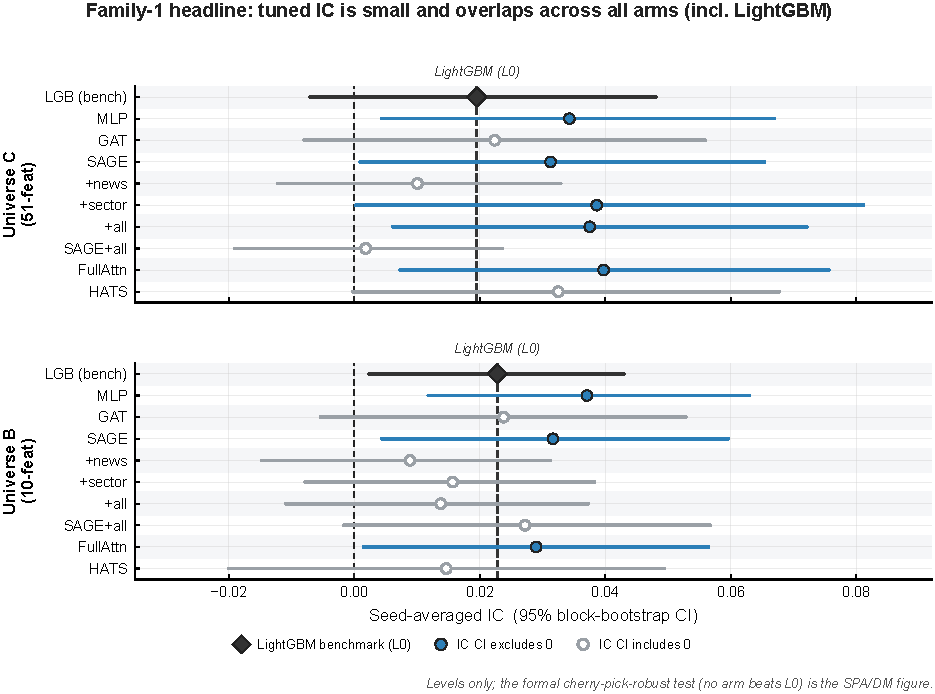
\includegraphics[width=.55\textwidth]{headline_ic_ladder}
  \caption{Per-arm pooled IC for the L0--L7 ladder. Intervals are 95\% stationary block-bootstrap CIs (block${}=21$\,d, 5000 reps); seeds${}=10$, folds${}=12$, benchmark${}={}$L0.}
  \label{fig:headline}
\end{figure}

\begin{table}[t]
  \begin{minipage}[t]{0.46\textwidth}
    \centering
    \caption{Per-arm pooled IC with 95\% block-bootstrap CI; ``e0'': CI excludes zero. The C/L5s Univ-C value ($0.0018$) is conditional on its \emph{defined} cells (27.5\% collapse to undefined IC, \S\ref{sec:stability}).}
    \label{tab:ic}
    \compacttable\setlength{\tabcolsep}{2.5pt}
    \begin{tabular}{@{}lccc c@{}}
      \toprule
      Rung & Univ B IC & e0 & Univ C IC & e0 \\
      \midrule
      L0 LightGBM & 0.0228 & y & 0.0195 & n \\
      L1 MLP      & 0.0371 & y & 0.0343 & y \\
      L2 GAT(corr)& 0.0238 & n & 0.0224 & n \\
      L2s SAGE    & 0.0317 & y & 0.0313 & y \\
      L3 +news    & 0.0089 & n & 0.0101 & n \\
      L4 +sector  & 0.0157 & n & 0.0386 & y \\
      L5 +both    & 0.0138 & n & 0.0375 & y \\
      L5s SAGE all& 0.0272 & n & 0.0018 & n \\
      L6 full-attn& 0.0290 & y & 0.0397 & y \\
      L7 HATS     & 0.0147 & n & 0.0325 & n \\
      \bottomrule
    \end{tabular}
  \end{minipage}\hfill
  \begin{minipage}[t]{0.51\textwidth}
    \centering
    \caption{DM/HLN pairwise ladder: seed-averaged daily $\Delta$IC and HLN $p$ ($^\ast$: BH-FDR reject at $q=0.05$ over the 20-test family). Near-equal $\Delta$IC can differ in $p$ as the daily-loss variance differs by universe.}
    \label{tab:dm}
    \compacttable\setlength{\tabcolsep}{3pt}
    \begin{tabular}{@{}l rr rr@{}}
      \toprule
      Pair (A$-$B) & B $\Delta$IC & B $p$ & C $\Delta$IC & C $p$ \\
      \midrule
      L1$-$L0 & $+0.0143$ & $0.052$ & $+0.0148$ & $0.011^\ast$ \\
      L2$-$L1 & $-0.0133$ & $<.001^\ast$ & $-0.0119$ & $<.001^\ast$ \\
      L6$-$L2 & $+0.0052$ & $0.356$ & $+0.0174$ & $0.001^\ast$ \\
      L7$-$L2 & $-0.0091$ & $0.195$ & $+0.0102$ & $0.002^\ast$ \\
      L2s$-$L2& $+0.0079$ & $0.118$ & $+0.0089$ & $<.001^\ast$ \\
      L3$-$L2 & $-0.0149$ & $0.006^\ast$ & $-0.0123$ & $0.009^\ast$ \\
      L4$-$L2 & $-0.0081$ & $0.227$ & $+0.0163$ & $0.012^\ast$ \\
      L5$-$L2 & $-0.0100$ & $0.110$ & $+0.0152$ & $<.001^\ast$ \\
      L5$-$L4 & $-0.0019$ & $0.172$ & $-0.0011$ & $0.831$ \\
      L5$-$L3 & $+0.0049$ & $0.066$ & $+0.0275$ & $<.001^\ast$ \\
      \bottomrule
    \end{tabular}
  \end{minipage}
\end{table}

\subsection{The predictive family: SPA and DM/HLN}\label{sec:spa}
Hansen's SPA test does not reject the null that no candidate beats LightGBM in either universe ($p_{\text{consistent}}=0.2767$ for B and $0.0774$ for C; $M=9$, $T=749$). In Universe~C the SPA bracket is $p_{\text{lower}}=0.055$, $p_{\text{consistent}}=p_{\text{upper}}=0.077$, so even the lower bound stays above 5\%, and the comparison is underpowered (observed gaps below the 80\% MDE); no tuned arm is confirmed to outperform tuned LightGBM after selection adjustment.

The local DM/HLN ladder gives a more detailed, but narrower, view of the same experiment (Figure~\ref{fig:spa}, Table~\ref{tab:dm}). Each layer is reported at its own error rate---SPA answers the global benchmark question; the DM ladder is pre-registered local evidence at its own FDR level---with no joint family-wise rate claimed. Two post-hoc sensitivities bound the layering: pooling all 26 $p$-values into one BH family rejects the same 11 DM contrasts and no Family-2 contrast, and Benjamini--Yekutieli~\citep{benjamini2001by}, valid under arbitrary dependence, keeps 7 of the 11---L2$-$L1 still rejects in \emph{both} universes, while C\,L1$-$L0, L3$-$L2 in both universes, and C\,L4$-$L2 drop; the first two are consistent with their suggestive and cost-sensitive labels (Appendix~\ref{app:robust}).

Within this tuned ladder, the strongest local evidence points to the non-graph MLP. In Universe~C the MLP beats LightGBM (L1$-$L0${}=+0.0148$), the correlation-GAT loses to the MLP (L2$-$L1${}=-0.0119$), and the tuned news-edge arm underperforms the correlation-GAT (L3$-$L2${}=-0.0123$; all BH-reject). These are local contrasts, not a global claim that graphs hurt: the sector, full-attention, HATS, and combined-edge arms all recover above the correlation-GAT in Universe~C, and the SPA non-rejection remains the selection-adjusted summary. The positive C\,L1$-$L0 contrast is only suggestive because the feature basis was leak-selected (Limitation~L1; the magnitude-matched Universe-B contrast, $+0.0143$, does not survive BH); the negative graph contrasts are less exposed---selection leakage can inflate apparent predictability but does not explain why the graph underperforms the MLP---and the L2$-$L1 penalty is BH-significant in the clean price-volume Universe~B as well ($\Delta$IC${}=-0.0133$).

Power is asymmetric: C\,L2$-$L1 exceeds its 80\% MDE whereas C\,L1$-$L0 falls below its own, so the data identify a detectable graph \emph{penalty} while leaving any benchmark-beating \emph{benefit} too small to detect at this sample size. Under-search of the graph arms at the fixed 30-trial budget (\S\ref{sec:data}) is an alternative reading, bounded by two observations: the same-budget, same-space arms L4 and L5 land \emph{above} L2 in Universe~C ($+0.0163$, $+0.0152$, both BH-reject), and the planted-signal control shows the stack converts graph-borne signal when present.

\begin{figure}[t]
  \centering
  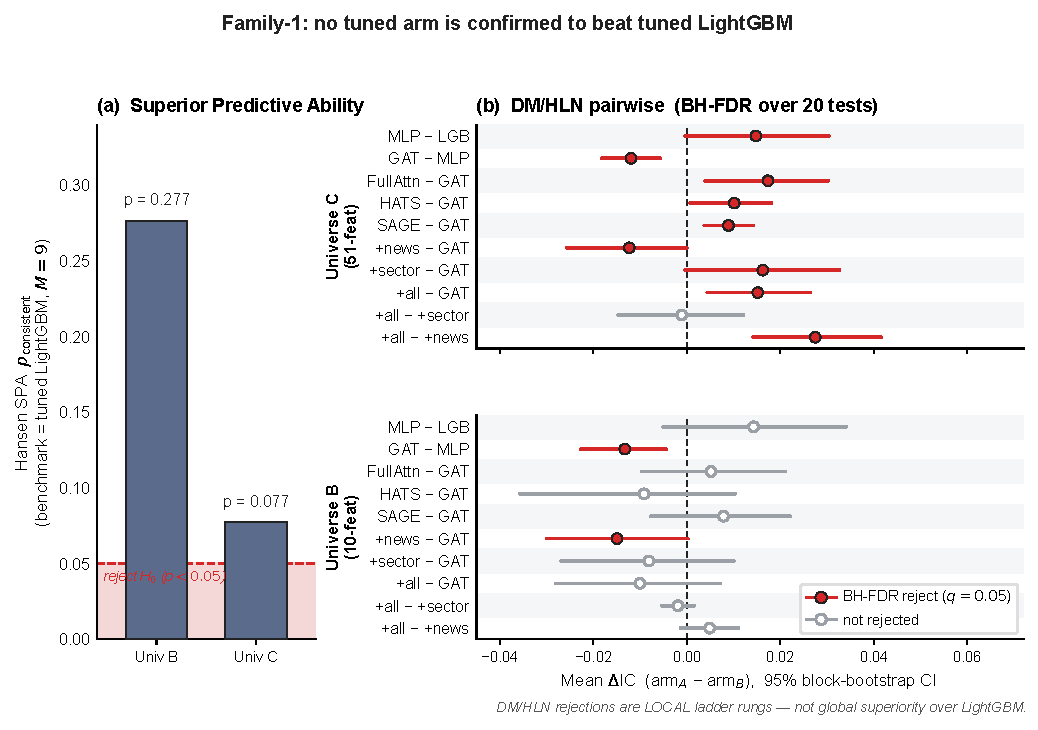
\includegraphics[width=.55\textwidth]{F9_spa_dm_confirmatory}
  \caption{SPA and local DM/HLN evidence. Left: SPA $p_{\text{consistent}}$ by universe. Right: 20 pre-registered DM/HLN contrasts, with filled markers denoting BH-FDR rejection at $q=0.05$.}
  \label{fig:spa}
\end{figure}

\paragraph{Regime concentration.} Pooled IC masks episodic predictability: most positive signal concentrates in a few quarters (especially 2024\,Q4 and 2025\,Q2), and roughly half of the test quarters are near zero or negative for almost every arm. This affects pooled IC \emph{levels} but not the load-bearing contrasts: none of the four BH-rejected ladder contrasts (L1$-$L0, L2$-$L1, L3$-$L2, L5$-$L3) changes sign in any leave-one-quarter-out (0/12, both universes) or leave-one-seed-out (0/10 each) replicate, with per-seed sign agreement between 8/10 and 10/10 (per-fold view and per-contrast counts in Appendices~\ref{app:diag} and~\ref{app:robust}).

\subsection{Net-of-cost crosswalk}\label{sec:cost}
We re-express each pre-registered ranking contrast under a 10\,bps net-of-cost convention (Table~\ref{tab:cost}, Figure~\ref{fig:cost}; descriptive, per the pre-registration in \S\ref{sec:families}). The two load-bearing Universe-C ladder contrasts (C\,L1$-$L0 and C\,L2$-$L1) survive this economic layer, with paired net $\Delta$Sharpe confidence intervals excluding zero; the edge-stacking contrast C\,L5$-$L3 also carries (a tuned-ladder pair: edge set and operating point change together); only the news-edge contrast C\,L3$-$L2 does not.

For L1$-$L0 the economic separation is larger than the IC gap suggests: at 10\,bps, over ${\approx}36$ rebalance returns, tuned LightGBM's net Sharpe is $-0.22$ (95\% CI $[-0.82,+0.36]$) against the MLP's $+0.95$ ($[+0.18,+1.77]$). Both level intervals are wide and overlap, so the load-bearing object is the \emph{paired} per-fold net $\Delta$Sharpe (Table~\ref{tab:cost}): its point estimate is $+1.17$ and its CI $[+0.36,+2.08]$---a stationary block-bootstrap interval over the 12 paired fold differences---excludes zero; it declines mildly with cost because the MLP turns over more (realized $L1$ turnover 2.90 versus 2.25 per rebalance in Universe~C).

The exception is C\,L3$-$L2: the news-edge rung underperforms the correlation-GAT in IC but not in net Sharpe (net $\Delta$Sharpe $+0.08$, CI $[-0.77,+0.89]$), so the news-edge IC underperformance is economically fragile---a local IC result, not a causal statement about news edges (\S\ref{sec:causal}). The crosswalk covers only Family-1 ranking pairs; Family-2 fixed-operating-point contrasts are evaluated only in IC.

\begin{table}[t]
  \centering
  \caption{Gross/net crosswalk for the load-bearing Universe-C ladder contrasts and the edge contrast C\,L5$-$L3. ``Carries?'': the gross-IC result reproduces in net Sharpe; ``CS'' (cost-sensitive): the net $\Delta$Sharpe CI straddles zero.}
  \label{tab:cost}
  \compacttable
  \begin{tabular}{@{}l r l c@{}}
    \toprule
    Pair & Gross $\Delta$IC (BH) & Net $\Delta$Sharpe@10\,bps [CI] & Carries? \\
    \midrule
    C L1$-$L0 & $+0.0148$ (r) & $+1.17\;[+0.36,+2.08]$ & yes \\
    C L2$-$L1 & $-0.0119$ (r) & $-0.72\;[-1.42,-0.10]$ & yes \\
    C L3$-$L2 & $-0.0123$ (r) & $+0.08\;[-0.77,+0.89]$ & no (CS) \\
    C L5$-$L3 & $+0.0275$ (r) & $+0.88\;[+0.12,+1.65]$ & yes \\
    \bottomrule
  \end{tabular}
\end{table}

\begin{figure}[t]
  \centering
  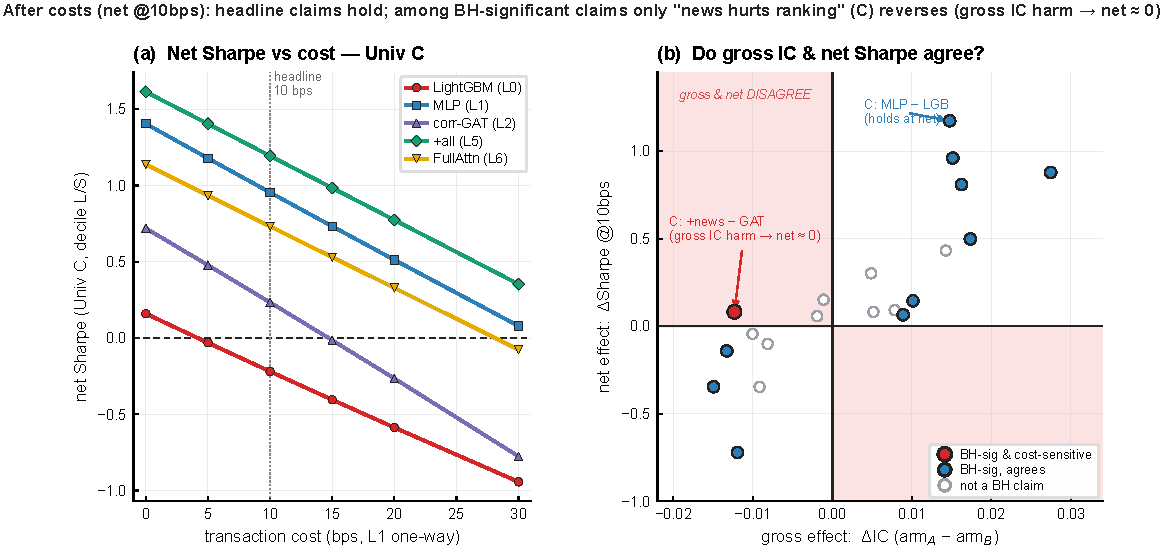
\includegraphics[width=.58\textwidth]{cost_gross_net}
  \caption{Net-of-cost crosswalk. Left: Universe-C cost ladder over 0--30\,bps. Right: sign agreement between gross IC and net Sharpe across the 20 pre-registered pairs, with C L3$-$L2 annotated.}
  \label{fig:cost}
\end{figure}

\subsection{The edge-attribution family: fixed-operating-point edges}\label{sec:causal}
Family-1's news-edge result mixes the edge change with changes in the tuned model; Family-2 evaluates each edge set at the frozen L2 hyperparameter vector (Table~\ref{tab:family2}, Figure~\ref{fig:family2}). None of the six contrasts survives BH-FDR, and all six are underpowered ($|$matched $\Delta$IC$|<$MDE@80\%); the point estimates are directionally positive, but not statistically reliable.

The sign reversals in Universe~B are suggestive but not conclusive: matched $\Delta$IC is positive where tuned $\Delta$IC was negative. In Universe~C, the sector ($+0.0137$) and sector$+$news ($+0.0141$) contrasts have the same sign as their tuned counterparts, while the news contrast is small and positive ($+0.0011$) despite a negative tuned rung ($-0.0123$). Thus, the fixed-operating-point test does not reproduce the tuned ladder's apparent news-edge harm; given low power, this is a failure to detect harm, not evidence that the edge is harmless.

\begin{figure}[t]
  \begin{minipage}[c]{0.48\textwidth}
    \centering
    \captionof{table}{Family-2 fixed-operating-point edge contrasts (matched $\Delta$IC, BH-FDR over 6). UP${}={}$underpowered.}
    \label{tab:family2}
    \compacttable\setlength{\tabcolsep}{2.5pt}
    \begin{tabular}{@{}ll r cc r@{}}
      \toprule
      Univ & Edge & Matched & BH & UP & Tuned \\
           &      & $\Delta$IC &   &    & $\Delta$IC \\
      \midrule
      B & news        & $+0.0015$ & n & y & $-0.0149$ \\
      B & sector      & $+0.0055$ & n & y & $-0.0081$ \\
      B & sector+news & $+0.0042$ & n & y & $-0.0100$ \\
      C & news        & $+0.0011$ & n & y & $-0.0123$ \\
      C & sector      & $+0.0137$ & n & y & $+0.0163$ \\
      C & sector+news & $+0.0141$ & n & y & $+0.0152$ \\
      \bottomrule
    \end{tabular}
  \end{minipage}\hfill
  \begin{minipage}[c]{0.48\textwidth}
    \centering
    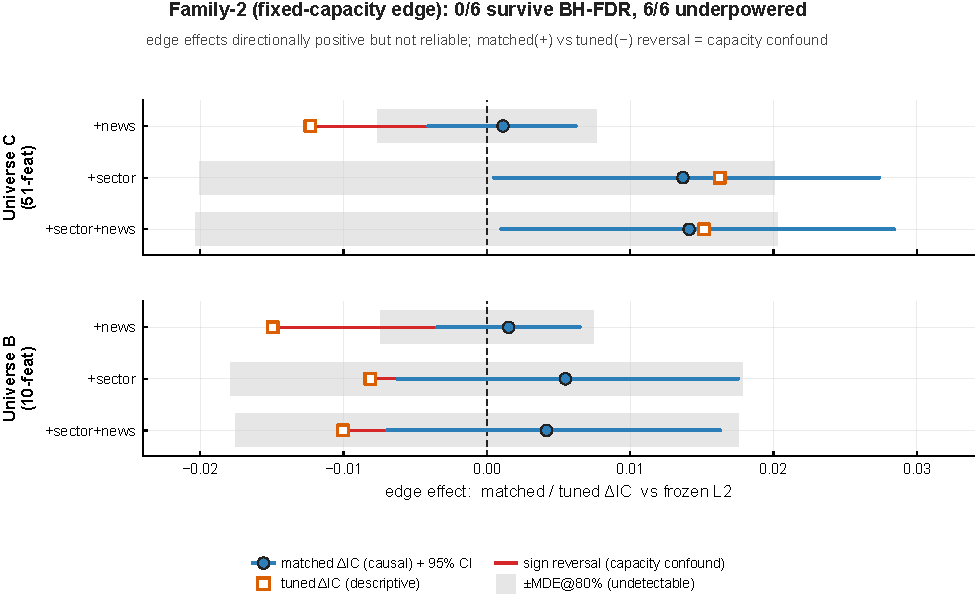
\includegraphics[width=\textwidth]{family2_edge_causal}
    \caption{Matched-$\Delta$IC versus tuned-$\Delta$IC for the six edge contrasts. The $\pm$MDE@80\% band contains every matched estimate, and no contrast survives BH-FDR.}
    \label{fig:family2}
  \end{minipage}
\end{figure}

\subsection{Disclosed failure modes}\label{sec:stability}
\emph{A tuned-configuration stability failure.} The Universe-C SAGE-Mean control arm with all edges (C/L5s) degenerates to constant predictions in 27.5\% of its test fold-seeds, leaving Spearman IC mathematically undefined in the affected cells; we treat undefined IC as missing rather than as a measured zero and do not retune only this losing arm. The main conclusion is unchanged: under exclusion, zero-fill, or zero-skill handling, C/L5s mean IC remains approximately zero and the Universe-C SPA $p$-value remains between $0.077$ and $0.080$. The cell-level breakdown and a plausible but unproven oversmoothing mechanism are detailed in Appendix~\ref{app:diag}.

\emph{Exploratory failure modes.} Two exploratory analyses outside the confirmatory families are detailed in Appendix~\ref{app:diag}: a loss-function horse race in which ListMLE showed a regime-shift inversion relative to the MSE loss later fixed for the ladder, and the audit of Universe-C's feature-basis leakage under strict $T-1$ re-ranking (Limitation~L1). Neither enters the confirmatory decision rules.

\section{Discussion}\label{sec:discussion}
The evidence does not show that GNNs fail: over this sample and protocol, with the graph path checked by a planted-signal control (\S\ref{sec:data}), no tuned arm is confirmed to beat a tuned tree benchmark, and the strongest local neural gain comes from the MLP.

The cleanest local DM contrast in both universes is L2$-$L1${}<0$: adding a correlation-GAT to the same node features reduces IC relative to the MLP; a $3\times$-budget trials sweep (Appendix~\ref{app:robust}) narrows but does not close this gap in the leak-free universe, so it is not merely an equal-budget artifact, even if exhaustive tuning fairness is not established. The C/L5s collapse offers one possible mechanism---dense-edge aggregation plus high dropout smoothing away cross-sectional signal---but only suggestively, since it is observed for SAGE-Mean with all edges, not for L2's sparse-correlation GAT; the claim is bounded to the correlation graph at the tuned operating point, not graph architectures in general.

The news-edge result shows why the two-family design matters: the tuned rung appears to harm ranking in Family-1, while the same edge change at the fixed L2 operating point is tiny, insignificant, and in Universe~B opposite-signed. The tuned ladder answers a deployment question, the fixed-operating-point arms an edge-attribution question subject to underfitting; conflating them would overstate an edge ablation.

\section{Limitations and Future Work}\label{sec:limits}
\textbf{(L1)} \emph{Selection-stage leakage in Universe-C's basis.} Universe~C's 51 columns come from Plan-AAA top-15 Alpha158 groups ranked under same-day OHLC; only 5 of the 15 groups survive strict $T-1$ re-ranking (Appendix~\ref{app:diag}). Runtime features are measured at $T-1$, but the basis \emph{selection} is leaked, so Universe-C positive results (MLP${}>{}$LightGBM, positive edge effects) are suggestive pending leak-free re-selection; null and negative within-universe contrasts are less exposed, since selection leakage inflates signal but does not explain graph underperformance.

\textbf{(L2)} Predictive skill concentrates in a minority of the 12 test quarters, so fold-level results are needed to interpret pooled IC. \textbf{(L3)} The C/L5s collapse is reported as a stability finding, not repaired by retuning. \textbf{(L4)} The LightGBM comparison is underpowered: no reliable evidence of superiority, not proven equality. \textbf{(L5)} Net Sharpe is descriptive, sensitive to heavy tails and turnover; interpretation should rely on fold-level paired $\Delta$Sharpe, and the equal-weight decile portfolio ignores liquidity and short-borrow costs, making net Sharpe an upper bound on realizable performance. \textbf{(L6)} L6 proxies the dense learned-attention family~\citep{li2024master,cheng2021adgat}, not learned-sparse architectures like FinMamba~\citep{finmamba2025}; LSTM/Transformer time encoders are not benchmarked. \textbf{(L7)} The evidence comes from one market and one prediction horizon.

\textbf{(L8)} \emph{Survivorship and non-point-in-time composition.} The universe is a fixed end-window survivor snapshot, not point-in-time (PIT) membership: a public-record audit identifies 87 departed window members (14.8\% of names, 8.2\% of PIT stock-days) and an 8.1\% look-ahead share from pre-addition inclusion---a 16.3\% two-sided mismatch. Pairing reduces mechanical cross-arm imbalance but does not make the estimand PIT and does not remove the look-ahead sampling bias; per-arm \emph{level} statements (Table~\ref{tab:ic}; \S\ref{sec:cost}) are unshielded and inflated---within-sample descriptive, not PIT-realizable, levels (full audit in Appendix~\ref{app:diag}). \textbf{(L9)} The correlation-graph hyperparameters ($|\rho|>0.6$, 126 days) are fixed, not ablated. Next steps: a point-in-time rebuild with delisting returns, a longer sample, cross-market replication, intraday news rebalancing, and learned-sparse architectures under the same protocol.

\subsection*{AI use statement}
Generative AI tools were used in this work, under the author's direction, to implement methods (experiment and analysis code), to clean and reformat data, to provide feedback on experimental methodology, and to support the analysis and interpretation of results. All AI-assisted code was reviewed and tested by the author, and all results, statistics, and claims were verified against the underlying experiment outputs. I take responsibility for the final content of this work, including text, claims, or artifacts produced with the aid of generative AI.

\subsection*{Ethics statement}
This study uses historical market data (prices, index membership, sector classifications, and news metadata) for a fixed universe of large-capitalization U.S. equities; it involves no human subjects, personal data, or user studies. The reported results are research findings on historical data under a specific evaluation protocol and do not constitute investment advice.

\subsection*{Reproducibility statement}
The project repository versions the code, confirmatory outputs, frozen tuned hyperparameters, the fold calendar, the Optuna grid, the ten seeds, and all analysis and figure scripts. The protocol and tuned hyperparameters were frozen before the confirmatory run, with the hyperparameter file identified by md5 \texttt{59ddd0a2} (\S\ref{sec:families}). A numeric-claim verifier checks the draft against underlying outputs, and the pre-registered protocol fixes the two-family decision rules. Experimental-setup details, including the DM/HLN estimator formulas, appear in Appendix~\ref{app:setup}, and additional robustness analyses in Appendix~\ref{app:robust}.

\ificlrfinal
\subsubsection*{Acknowledgments}
I am grateful to Professor Jinchi Lv (USC Marshall, Data Sciences and Operations) for his supervision and guidance throughout this project. All errors are my own.
\fi

\bibliography{references}
\bibliographystyle{iclr2027_conference}

\appendix
% ============================================================================
% Appendix: Experimental setup details
% Every number below is copied verbatim from the cited source file; see the
% per-table / per-sentence "% source:" comments.
% ============================================================================
\section{Experimental setup details}\label{app:setup}

\subsection{Walk-forward fold calendar}\label{app:setup:folds}

% source: paper/main.tex, subsection "Walk-forward cross-validation" (line 121);
%         docs/storya_paper_draft_v2.md §3.1
Our validation design is a 12-fold \emph{expanding-window walk-forward}. In fold $k$, training ends at a quarter boundary, validation is the next quarter, and testing is the following quarter. The twelve test quarters run from 2023\,Q1 through 2025\,Q4, yielding $T=749$ pooled test days. Because the label is a 21-trading-day forward return, we purge the final 21 training days to eliminate label overlap \citep{lopezdeprado2018advances}. A secondary sliding 252-day specification is a robustness exercise only, opening no additional inferential family.
% source: paper/main.tex line 158 (histories span)
Price, sector, and news histories span 2021 through 2026.

% source: docs/storya_paper_draft_v2.md, Supplementary §S1, Table ST1a (lines 329-338);
%         test-day counts from experiments/storya_v21_main12_tuned/results.csv,
%         n_test_days summed over the 12 folds (as cited in ST1a)
\begin{table}[h]
  \centering
  \caption{Walk-forward fold calendar. Twelve expanding-window folds; each test quarter follows a one-quarter validation set and a 21-day purge embargo. Pooled test span is $T=749$ trading days.}
  \label{app:setup:tab:folds}
  \begin{tabular}{rlr@{\hspace{2em}}rlr}
    \toprule
    Fold & Test quarter & Test days & Fold & Test quarter & Test days \\
    \midrule
    0 & 2023 Q1 & 62 & 6  & 2024 Q3 & 64 \\
    1 & 2023 Q2 & 62 & 7  & 2024 Q4 & 64 \\
    2 & 2023 Q3 & 63 & 8  & 2025 Q1 & 60 \\
    3 & 2023 Q4 & 63 & 9  & 2025 Q2 & 62 \\
    4 & 2024 Q1 & 61 & 10 & 2025 Q3 & 64 \\
    5 & 2024 Q2 & 63 & 11 & 2025 Q4 & 61 \\
    \bottomrule
  \end{tabular}
\end{table}

\subsection{Hyperparameter search space}\label{app:setup:grid}

% source: docs/storya_paper_draft_v2.md, Supplementary §S1, Table ST1b (lines 340-366)
%         and §4.3 (line 140); underlying protocol: docs/protocol_v2_freeze.md §4
Every ladder rung is tuned independently with Optuna, $N=30$ trials per arm under an equal compute budget and six hyperparameter dimensions per family. Search centres are the pilot defaults, so the pilot is the $N=1$ centre sample and remains comparable. Fixed (not tuned) for the neural arms: epochs${}=100$, patience${}=15$, gradient accumulation${}=32$; HATS relations${}=3$ (\texttt{linear\_shared}; the three relation types are correlation, GICS sector, and news co-occurrence, feeding a 21-day ranking head).
% source: docs/storya_paper_draft_v2.md line 366
The LightGBM grid is six-dimensional to match the neural dimension count and preserve an equal tuning budget for the benchmark.

% source: docs/storya_paper_draft_v2.md, Table ST1b (both panels, verbatim)
\begin{table}[h]
  \centering
  \caption{Hyperparameter search grid (Optuna, $N=30$ trials per arm). Top panel: neural arms (MLP / GAT / L6 full-attention / L7 HATS). Bottom panel: LightGBM (L0).}
  \label{app:setup:tab:grid}
  {\small
  \setlength{\tabcolsep}{4pt}
  \begin{tabular}{lll}
    \toprule
    Dimension & Centre & Search range \\
    \midrule
    \multicolumn{3}{l}{\emph{Neural arms}} \\
    learning rate    & $1\times10^{-3}$ & log-uniform $[1\times10^{-4},\,1\times10^{-2}]$ \\
    weight decay     & $1\times10^{-4}$ & log-uniform $[1\times10^{-5},\,1\times10^{-3}]$ \\
    dropout          & $0.3$            & $\{0.1,\,0.2,\,0.3,\,0.5\}$ \\
    hidden channels  & $64$             & $\{32,\,64,\,128\}$ \\
    num layers       & $2$              & $\{1,\,2,\,3\}$ \\
    attention heads  & $4$              & $\{2,\,4,\,8\}$ \\
    \midrule
    \multicolumn{3}{l}{\emph{LightGBM (L0)}} \\
    num leaves        & $31$             & $\{15,\,31,\,63,\,127\}$ \\
    learning rate     & $0.05$           & log-uniform $[0.01,\,0.1]$ \\
    min data in leaf  & $20$             & $\{10,\,20,\,50,\,100\}$ \\
    n estimators      & $100$            & early-stopped (not gridded) \\
    \texttt{lambda\_l1} & $1\times10^{-8}$ & log-uniform $[1\times10^{-8},\,1.0]$ \\
    \texttt{lambda\_l2} & $1\times10^{-8}$ & log-uniform $[1\times10^{-8},\,1.0]$ \\
    \bottomrule
  \end{tabular}
  }
\end{table}

\subsection{Frozen tuned hyperparameters}\label{app:setup:frozen}

% source: paper/main.tex, subsection "Pre-registration" (line 154);
%         docs/storya_paper_draft_v2.md §3.4 (line 120) and §8 (line 323)
The protocol and tuned hyperparameters were frozen before the confirmatory run, with the hyperparameter file identified by md5 \texttt{59ddd0a2} (\texttt{artifacts/storya\_v21\_tune/frozen\_hparams.json}, committed to the repository before launch). Table~\ref{app:setup:tab:frozen} reports the discrete winning hyperparameters of each of the 20 tuning studies verbatim from the frozen file; the continuous winners (learning rate and weight decay) are recorded there at full floating-point precision and are not re-rounded here.
% source: artifacts/storya_v21_tune/frozen_hparams.json, studies B_L0 and C_L0, winner_params
For L0 (LightGBM), the frozen discrete winners are \texttt{num\_leaves}${}=15$ with \texttt{min\_data\_in\_leaf}${}=50$ in Universe~B and \texttt{num\_leaves}${}=15$ with \texttt{min\_data\_in\_leaf}${}=100$ in Universe~C.
% source: artifacts/storya_v21_tune/frozen_hparams.json, n_trials fields of C_L5s (25) and C_L6 (29)
The frozen file records \texttt{n\_trials}${}=25$ for study C/L5s and $29$ for C/L6; all other studies record $30$.

% source: artifacts/storya_v21_tune/frozen_hparams.json (30-trial studies, winner_params, verbatim);
%         dagger rows: artifacts/storya_v21_tune/frozen_hparams_m14.json, studies B_L2 and C_L2 (n_trials=90)
\begin{table}[h]
  \centering
  \caption{Frozen tuned discrete hyperparameters per neural tuning study (verbatim from \texttt{frozen\_hparams.json}, md5 \texttt{59ddd0a2}). Arm definitions follow the model ladder in the main text; ``--'' marks a dimension that is not part of the arm's recorded winner. $^{\dagger}$~rows are the 90-trial L2 re-tunes from the M14 search-budget sensitivity (\texttt{frozen\_hparams\_m14.json}); all other arms are unchanged at 30 trials.}
  \label{app:setup:tab:frozen}
  {\small
  \setlength{\tabcolsep}{4pt}
  \begin{tabular}{llrrrrr@{\hspace{2em}}llrrrrr}
    \toprule
    Univ. & Arm & Drop. & Hid. & Lay. & Heads & Trials & Univ. & Arm & Drop. & Hid. & Lay. & Heads & Trials \\
    \midrule
    B & L1  & 0.3 & 128 & 3 & --  & 30 & C & L1  & 0.1 & 128 & 1 & --  & 30 \\
    B & L2  & 0.3 & 64  & 2 & 2   & 30 & C & L2  & 0.1 & 128 & 1 & 4   & 30 \\
    B & L2s & 0.3 & 128 & 1 & --  & 30 & C & L2s & 0.1 & 128 & 1 & --  & 30 \\
    B & L3  & 0.2 & 32  & 2 & 4   & 30 & C & L3  & 0.1 & 32  & 2 & 2   & 30 \\
    B & L4  & 0.1 & 32  & 2 & 4   & 30 & C & L4  & 0.2 & 128 & 1 & 4   & 30 \\
    B & L5  & 0.1 & 32  & 2 & 4   & 30 & C & L5  & 0.1 & 128 & 1 & 4   & 30 \\
    B & L5s & 0.1 & 64  & 1 & --  & 30 & C & L5s & 0.5 & 32  & 3 & --  & 25 \\
    B & L6  & 0.1 & 32  & 2 & 8   & 30 & C & L6  & 0.1 & 64  & 1 & 4   & 29 \\
    B & L7  & 0.3 & 128 & 1 & 2   & 30 & C & L7  & 0.1 & 128 & 1 & 4   & 30 \\
    \midrule
    B & L2$^{\dagger}$ & 0.1 & 32 & 1 & 2 & 90 & C & L2$^{\dagger}$ & 0.1 & 128 & 1 & 8 & 90 \\
    \bottomrule
  \end{tabular}
  }
\end{table}

% source: paper/main.tex line 166 (trials-sensitivity sweep, verbatim numbers and hedging);
%         artifacts/storya_v21_tune/frozen_hparams_m14.json, meta_m14 field
Equal budget equalizes trial count, not search adequacy. Neural arms have higher-dimensional spaces than LightGBM, a caveat for the ``MLP beats GAT'' interpretation. A trials-sensitivity sweep probes it: re-tuning L2 at $3\times$ the budget (90 trials, matching the MLP's search density) leaves the leak-free Universe-B penalty significant (L2$-$L1${}=-0.0090$, HLN $p=0.002$, BH-reject) but drops Universe-C's below significance ($-0.0069$, $p=0.059$, sign unchanged); the gap narrows without closing, so the primary leak-free result is not an equal-budget artifact.

\subsection{Cell budget accounting}\label{app:setup:cells}

% source: docs/storya_paper_draft_v2.md §4.4 (line 161) and Table ST1c (line 368);
%         paper/main.tex line 170
The confirmatory main table is 2160 cells for the nine non-HATS rungs ($9$ arms${}\times{}2$ universes${}\times{}12$ folds${}\times{}10$ seeds), plus 240 L7/HATS cells, plus 720 fixed-capacity Family-2 cells (L3fc/L4fc/L5fc${}\times{}2\times{}12\times{}10$), for 3120 cells in total. Each of these three stores is internally complete (0 failed, 0 duplicate \texttt{cell\_id}) and is consumed separately by its pre-specified family: Family-1 reads the main table plus L7, and Family-2 reads the fixed-capacity store. The fixed-capacity arms reuse the main per-arm \texttt{cell\_id} numbering by design, so the three stores are not concatenated into one global key space.
% source: docs/storya_paper_draft_v2.md §4.4 (line 161), incl. family1_summary.md citation
The L7 contingency rule --- an automatic health gate that demotes HATS out of the family if more than 20\% of its cells diverge or collapse --- was not triggered (diverge fraction 0, collapse fraction 0; source \texttt{family1\_summary.md}), so L7 stays in the family and SPA runs at $M=9$.

% source: docs/storya_paper_draft_v2.md, Table ST1c (line 368): seeds and feature counts
The ten canonical seeds, used in all experiments, are $\{7,\,34,\,86,\,99,\,123,\,456,\,789,\,1024,\,2024,\,2026\}$. Universe~B carries 10 features and Universe~C carries 51, all measured strictly at $T-1$.

\subsection{News-graph construction}\label{app:setup:news}

% source: paper/main.tex (acmart), SS Data and Setup news-graph sentence (moved here in the ICLR conversion)
The news graph fits no construction parameters: ticker tags are the provider's per-article annotations, an edge requires only co-mention in a multi-ticker article, and the only temporal parameter is the daily cutoff---the article's publication timestamp must fall before the NYSE close on $T-1$. Nothing is estimated from full-sample or future data.

\subsection{DM/HLN estimator details}\label{app:setup:dmhln}

% source: paper/main.tex line 139 (contrast family, verbatim)
Local paired evidence comes from Diebold--Mariano tests \citep{diebold1995comparing} with the Harvey--Leybourne--Newbold small-sample correction \citep{harvey1997testing} on 20 pre-registered contrasts: five ladder contrasts, $\{$L1$-$L0, L2$-$L1, L6$-$L2, L7$-$L2, L2s$-$L2$\}$, and five edge-set contrasts, $\{$L3$-$L2, L4$-$L2, L5$-$L2, L5$-$L4, L5$-$L3$\}$, each in both universes. The main correction is BH-FDR at $q=0.05$ over the pooled 20-test family \citep{benjamini1995controlling}. A per-universe BH correction gives the same rejection decisions.

% source: paper/main.tex line 141 (estimator paragraph, reproduced faithfully; moved from main text)
The DM statistic uses Newey--West HAC standard errors \citep{newey1987simple} with the Newey--West (1994) data-driven bandwidth $L=\lfloor 4(T/100)^{2/9}\rfloor$ ($L=6$ at $T=749$) to absorb serial correlation in the daily loss differential. The HLN factor, $\sqrt{(T+1-2h+h(h-1)/T)/T}$ with $h=21$, is a separate small-sample $t$-correction for the $h$-step forecast horizon, not a second autocorrelation adjustment. The two operate on different margins, the HAC long-run variance and the small-sample degrees of freedom, and are therefore not double-counted; the small-sample factor is conservative.

% source: docs/storya_paper_draft_v2.md §3.3 (line 110), secondary fixed-lag column
A secondary \texttt{HLN\_p\_t\_lag21} column is reported so that marginal rungs are not called robust without checking a fixed-lag HAC.


% ----------------------------------------------------------------------
% Appendix fragment: Extended related work and evaluation-protocol audit.
% Sources of all cells and numbers (repo-relative):
%   docs/lit_benchmark_2026-07-03.md  (15-paper benchmark: SS3 per-paper
%     summaries, SS5 comparison matrix, SS5.1 findings, SS6 evaluation)
%   docs/storya_paper_draft_v2.md SS2.3 (Table T8 + framing sentence)
%   paper/main.tex (our protocol facts and bounded-claim wording)
% Convention: "n.r." = not reported in the cited paper. No number below is
% computed or extrapolated; each is copied verbatim from the named source.
% ----------------------------------------------------------------------
\section{Extended related work and evaluation-protocol audit}\label{app:lit}

% source: docs/lit_benchmark_2026-07-03.md, SS1 (inclusion criteria, final 15, exclusion log)
This appendix expands the related-work discussion in the main text with an audit of the evaluation protocols \emph{reported} by the eight most closely related deep-learning systems for cross-sectional stock ranking, published between 2019 and 2024 at TOIS, AAAI, KDD, and CIKM: RSR \citep{feng2019temporal}, STHAN-SR \citep{sawhney2021sthansr}, AD-GAT \citep{cheng2021adgat}, TRA \citep{lin2021tra}, THGNN \citep{thgnn2022}, MASTER \citep{li2024master}, StockMixer \citep{fan2024stockmixer}, and MDGNN \citep{qian2024mdgnn}. TRA is not graph-based but is included as the closest published Qlib-based ranking baseline; HATS \citep{kim2019hats} and FinMamba \citep{finmamba2025}, which motivate rungs of our ladder, are excluded from the audit because neither is published at an archival venue. All entries were compiled from the papers as published. Throughout, an entry records what a paper \emph{reports}: ``n.r.''\ marks a property a paper does not report, not a claim that the property is impossible for the method, and we treat every gap as a reporting difference, not as evidence that earlier methods could not be evaluated under this protocol.

\subsection{Protocol comparison matrix}\label{app:lit:matrix}

% Table sources, row by row (docs/lit_benchmark_2026-07-03.md):
%   RSR:        SS5 matrix row "RSR (TOIS'19)"; universe from SS3 "RSR" (NASDAQ 1,026 / NYSE 1,737)
%   STHAN-SR:   SS5 row "STHAN-SR (AAAI'21)"; universe from SS3 (NASDAQ, NYSE, TSE)
%   AD-GAT:     SS5 row "AD-GAT (AAAI'21)"; universe from SS3 (S&P 500 filtered to 198)
%   TRA:        SS5 row "TRA (KDD'21)"; universe from SS3 (CSI800)
%   THGNN:      SS5 row "THGNN (CIKM'22)"; universe from SS3 (S&P 500 + CSI 300)
%   MASTER:     SS5 row "MASTER (AAAI'24)"; universe from SS3 (CSI300 + CSI800)
%   StockMixer: SS5 row "StockMixer (AAAI'24)"; universe from SS3 (NASDAQ + NYSE + S&P500 474)
%   MDGNN:      SS5 row "MDGNN (AAAI'24)"; universe from SS3 (CSI 100 + CSI 300); seeds "not reported"
%   This work:  SS5 row "Ours"; universe 501 names from SS2 profile; cost grid {0,5,10,15,20,30} bps from SS2
\begin{table}[t]
\centering
\caption{Evaluation-protocol audit of the eight most closely related deep/GNN cross-sectional ranking systems and this work. Cells reflect each paper's \emph{reported} protocol; ``n.r.''\ marks a property the paper does not report, not a claim that the property is impossible for the method, and the table records reporting differences, not evidence that prior methods could not be evaluated under this protocol. Universe counts, where shown in parentheses, are numbers of stocks. Costs: no audited paper models transaction costs; RSR and THGNN explicitly dismiss them, and AD-GAT reports no portfolio backtest at all. Seeds: AD-GAT's entry is the mean of the top five of 30 initializations \emph{selected on validation}; TRA and MASTER additionally report standard deviations over their five seeds. Graph-off: ``yes''/``no''/``partial'' indicates whether the paper reports a no-graph variant of its own framework (details in \S\ref{app:lit:papers}); ``n/a'' marks the non-graph TRA. The final row abbreviates our protocol: 12-fold expanding walk-forward with a 21-day purge; ten seeds plus a leave-one-seed-out (LOSO) check; BH-FDR at $q=0.05$ with Benjamini--Yekutieli and pooled-26 sensitivities; a 0--30\,bps cost grid with per-arm, per-fold turnover; and the feature-matched L2$-$L1 graph-off contrast as the headline, complemented by the fixed-operating-point edge-attribution family. Full citations for the audited systems appear in the opening paragraph of this appendix.}
\label{app:lit:tab-matrix}
{\small
\setlength{\tabcolsep}{3pt}
\begin{tabular}{@{}lllllll@{}}
\toprule
Work & Universe & Splits & Seeds & Mult. & Costs & Graph-off \\
\midrule
RSR & NASDAQ/NYSE & single (2017) & 5 & none & none & yes \\
STHAN-SR & NASDAQ/NYSE/TSE & single ($\times$3) & 5 & none & none & yes \\
AD-GAT & S\&P500 (198) & single (70d) & top-5/30 & none & none & no \\
TRA & CSI800 & single, purged & 5 & none & none & n/a \\
THGNN & S\&P500/CSI300 & single (2020) & 5 & none & none & no \\
MASTER & CSI300/CSI800 & single (10q) & 5 & none & none & no \\
StockMixer & NASDAQ/NYSE/S\&P & single ($\times$3) & 3 & none & none & partial \\
MDGNN & CSI100/CSI300 & 7 rolling folds & n.r. & none & none & no \\
\midrule
This work & S\&P500 (501) & 12-fold WF & 10+LOSO & BH+BY & 0--30\,bps & matched L2$-$L1 \\
\bottomrule
\end{tabular}}
\end{table}

% source: docs/lit_benchmark_2026-07-03.md, SS5.1 findings 1-4
% (7/8 single split; MDGNN 7 rolling folds; 0/8 multiple-testing correction while
%  comparing 8-15 models x 3-6 metrics x 2-3 markets; 0/8 costs, RSR & THGNN dismiss;
%  4/8 no hypothesis test, other 4 uncorrected t/Wilcoxon vs 1-2 references;
%  seed mode 5, min 3 (StockMixer), one unreported (MDGNN); no LOSO in any paper)
% and SS6.1 dominance table (pre-registration 0/8; power analysis 0/8; positive control 0/8)
Three aggregate facts stand out in Table~\ref{app:lit:tab-matrix}. First, seven of the eight papers evaluate on a single chronological split; MDGNN alone uses seven rolling folds, and only TRA adds purge gaps. Second, none of the eight applies any multiple-testing correction, although the papers typically compare on the order of 8--15 models across 3--6 metrics and 2--3 markets; four of the eight report no hypothesis test at all, and the remaining four use uncorrected $t$ or Wilcoxon tests against one or two reference models. Third, none of the eight models transaction costs; RSR and THGNN dismiss them explicitly. Seed counts cluster at five (minimum three; one paper does not report seeds), and no audited paper reports a leave-one-seed-out check, a pre-registered analysis plan, a power analysis, or a planted-signal positive control.

\subsection{Per-paper positioning}\label{app:lit:papers}

% source: docs/lit_benchmark_2026-07-03.md SS3 "THGNN" (trailing 20-day correlation, |rho|>=0.6,
% regenerated daily; single test year 2020 per market; 5 repeated tests; no significance tests;
% costs explicitly ignored; all ablations retain the graph) and SS5.1 finding 8;
% our alpha-1 spec from paper/main.tex ("126-day rolling Spearman-correlation graph, refreshed
% every 21 days from training data only, with an edge when |rho|>0.6")
\paragraph{THGNN \citep{thgnn2022}.} Among the eight systems, THGNN has the cleanest graph construction: its edges are regenerated daily from a trailing 20-day return correlation with a $|\rho|\ge 0.6$ threshold, a construction that, as described, uses no future or full-sample information. This specification is nearly identical to our $\alpha$1 graph (a trailing 126-day rolling Spearman correlation, refreshed every 21 days from training data only, with an edge when $|\rho|>0.6$), so the edge type stressed by our headline feature-matched contrast is the one this recent state-of-the-art system actually relies on, not a strawman. THGNN's evaluation, however, uses a single test year (calendar 2020) per market with five repeated runs, no significance tests, and explicitly ignored costs, and all of its reported ablations retain the graph, so the framework has no internal no-graph variant. The two studies also differ in label, horizon, and period, so we read the connection as positioning, not replication.

% source: docs/lit_benchmark_2026-07-03.md SS3 "RSR" (Wikidata single snapshot across train and
% 2017 test; survivorship-style universe filter; ablation: Rank_LSTM 0.68 vs GCN 0.24, RSR_E
% industry 0.20, RSR_I industry 0.23, Wiki RSR_I 1.19, IRR = top-1 daily buy-hold-sell) and
% SS3 "STHAN-SR" (static Wikidata through test incl. TSE to 08/2020; LSTM-only SR 0.95 vs full
% 1.42; hypergraph conv w/o attention 0.93) and SS6.1 look-ahead note
\paragraph{RSR \citep{feng2019temporal} and STHAN-SR \citep{sawhney2021sthansr}.} Both works attach relation graphs built from a single Wikidata snapshot, mined at collection time and held fixed through the test period (in STHAN-SR's case including a TSE test extending to August 2020); neither paper discusses the resulting look-ahead exposure in graph construction, and RSR additionally restricts its universe to stocks with near-complete full-sample histories, a survivorship-style filter. By contrast, our news graph is strictly point-in-time (publication-timestamp gated) and our correlation graph is trailing-only. Notably, both papers' own ablations already contain mixed graph-off evidence: in RSR, the no-graph Rank\_LSTM attains a NASDAQ investment return ratio of 0.68, above the GCN variant (0.24) and both industry-relation RSR variants (0.20 and 0.23), with only the Wikidata-relation RSR\_I variant (1.19) exceeding it; in STHAN-SR, the plain hypergraph convolution without attention (Sharpe 0.93) trails the LSTM-only variant (0.95), while the full model reaches 1.42. The seminal papers' internal evidence is thus consistent with a configuration-conditional rather than uniform graph benefit; our contribution is to measure that conditionality under controlled inference.

% source: docs/lit_benchmark_2026-07-03.md SS3 "AD-GAT" (198 stocks retained by no-missing-data
% + >=100 news articles over the full period; single 560/70/70-day split with one 70-day test
% window; 30 inits, top 5 selected by validation, mean of the 5 reported; DA/AUC only, no
% backtest; uncorrected t-tests) and SS6.1 selective-reporting note
\paragraph{AD-GAT \citep{cheng2021adgat}.} AD-GAT evaluates on an S\&P~500 subset of 198 stocks retained by requiring no missing data and at least 100 news articles over the full sample period, a coverage filter that conditions on future information, and its single split leaves one 70-day test window. It trains 30 initializations and reports the mean of the top five selected on validation, together with direction-accuracy and AUC only (no portfolio backtest) and uncorrected $t$-tests. Relative to a deployment estimand, this run-selection protocol yields an upward-biased estimate of test performance; our seed-mean estimand with a leave-one-seed-out check is designed as the opposite convention. We record this as a difference in reported estimands, not as an error in the paper's own terms.

% source: docs/lit_benchmark_2026-07-03.md SS3 "KMZ" (RFF up to P=12,000; OOS timing Sharpe gain
% ~0.47/yr at t~3 while R2_oos substantially negative, e.g. -3.8% with Sharpe 0.46; single risky
% asset) and SS6.3 item 3 (our GAT arms hidden 32-64, <=2 layers, not in the P>T ridge regime);
% bounded-claim wording from paper/main.tex ("the correlation graph at the tuned operating
% point, not graph architectures in general"); net Sharpe descriptive per paper/main.tex
\paragraph{The complexity counterpoint.} The virtue-of-complexity results of \citet{kmz2024jf} are the strongest published counterweight to any ``simple beats complex'' reading of our findings: random-feature ridge models with up to $P=12{,}000$ features deliver an out-of-sample market-timing Sharpe gain of approximately 0.47 per year ($t\approx3$) even while out-of-sample $R^2$ remains substantially negative (e.g., $-3.8\%$ alongside a Sharpe ratio of 0.46). Their setting, however, is single-asset market timing in the heavily shrunk $P>T$ regime, whereas our equal-budget tuned ladder compares standard GNN architectures at tuned operating points (hidden sizes 32--64, at most two layers) far from that regime. The two sets of results therefore do not contradict each other: our negative graph contrast is bounded to the correlation graph at the tuned operating point, not graph architectures in general, and is silent about over-parameterized models under ridge shrinkage. Their argument that $R^2$-type fit measures are incomplete guides to economic value is also consistent with our choice to report net Sharpe alongside IC, with IC remaining the only confirmatory metric and the net-Sharpe layer descriptive.

% source: docs/lit_benchmark_2026-07-03.md SS3 "JKP" (153 factors x 93 countries; replication-rate
% sequence 35% HXZ-style -> 55.6% their construction -> 82.4% CAPM alpha -> 75.6% BY -> 82.4%
% Bayesian; ~45pp swing per SS6.3 item "the MT framework choice can move headline conclusions by
% ~45pp"); BY sensitivity outcome from paper/main.tex ("keeps 7 of the 11 --- L2-L1 still rejects
% in both universes, while C L1-L0 and L3-L2 drop")
\paragraph{Factor-zoo multiplicity.} Studying 153 factors across 93 countries, \citet{jkp2023jf} show that the multiple-testing framework alone can move a headline replication rate by roughly 45 percentage points: from 35\% under an HXZ-style construction, to 55.6\% under their capped value-weighted construction, to 82.4\% under a CAPM-alpha test object, with 75.6\% under frequentist Benjamini--Yekutieli control and 82.4\% under their hierarchical Bayesian model. Their hierarchical empirical-Bayes treatment of correlated signals is more powerful than BH/BY and can rescue borderline findings. Our design deliberately takes the conservative frequentist direction, pre-registered BH families with a Benjamini--Yekutieli sensitivity valid under arbitrary dependence, under which 7 of our 11 BH-rejected ladder contrasts survive: the graph-penalty contrast L2$-$L1 still rejects in both universes, while the weaker C\,L1$-$L0 and L3$-$L2 contrasts drop. A joint Bayesian treatment of the correlated ladder contrasts, in their spirit, is a natural extension that we leave to future work; because our choice errs in the stricter direction, our surviving results are robust to it.

\subsection{What the matrix implies for reported GNN gains}\label{app:lit:implications}

% source: docs/lit_benchmark_2026-07-03.md SS5.1 findings 3-6 (0/8 multiplicity control while
% comparing 8-15 models x 3-6 metrics x 2-3 markets; daily top-k rotation implies near-100%
% daily turnover; RSR/STHAN-SR internal graph-off evidence mixed; StockMixer MLP-family beats
% GNN hybrids under single-split/3-seed/no-cost protocol) and SS3 "GNN survey" (CSUR survey
% reports no prevalence counts of significance testing, costs, seeds); "suggestive" label for
% our MLP result and "non-rejection, not evidence that the models are equal" from paper/main.tex
Read as a whole, the matrix supports a bounded caution rather than a refutation. Because none of the eight audited papers corrects for multiplicity while comparing on the order of 8--15 models across 3--6 metrics and 2--3 markets, the reported margins carry unquantified selection effects; because none models costs while relying on daily top-$k$ rotation portfolios that imply near-100\% daily turnover, gross performance gaps need not survive frictions; and where internal graph-off evidence exists (RSR, STHAN-SR), it already points to a configuration-conditional benefit. None of this shows that any specific published gain is spurious---the audited papers follow the reporting norms of their venues and periods---but it does mean the published record, as reported, cannot bound how much of the headline gains would survive a multi-seed, multiplicity-controlled, cost-aware re-evaluation. Two independent observations are at least consistent with our findings: StockMixer, an MLP-family architecture, is reported to outperform GNN hybrids on the field's own benchmark datasets \citep{fan2024stockmixer}, converging with our (suggestive) non-graph MLP result, though under the same single-split, three-seed, cost-free protocol; and the field's systematic review \citep{patel2024survey} catalogues architectures without tabulating the prevalence of significance testing, cost modeling, or seed reporting, so the rigor gap this audit measures had not previously been quantified. We apply the same standard to our own results: the SPA outcome is a non-rejection, not evidence that the models are equal, and the graph-penalty finding is bounded to the correlation graph at the tuned operating point, not graph architectures in general.


% ======================================================================
% Appendix: Additional robustness analyses (ICLR 2027 version)
% Pure fragment: no preamble, no \begin{document}.
% Every number below is copied verbatim from the cited source file;
% see the "% source:" comment above each table / number-bearing passage.
% ======================================================================
\section{Additional robustness analyses}\label{app:robust}

% source: docs/analysis.md, entry 2026-07-02-a (positioning: post-hoc sensitivity,
% not a new confirmatory family, does not replace the two pre-registered families)
The analyses in this appendix are post-hoc sensitivities and one pre-confirmatory
pipeline control. They supplement the two pre-registered confirmatory families;
they are not new confirmatory families and do not replace the pre-registered
decision rules.

\subsection{Trials-sensitivity of the correlation-GAT penalty}\label{app:robust:trials}

\paragraph{Motivation.}
% source: docs/analysis.md, entry 2026-07-03-a (Motivation): 108 vs 36 combos,
% extra gat_heads dimension, 3x categorical space
The equal 30-trial tuning budget equalizes trial count, not search adequacy. The
correlation-GAT's categorical hyperparameter space is three times the MLP's---the
extra attention-heads dimension yields 108 versus 36 combinations---so the finding
that the tuned correlation-GAT (L2) underperforms the tuned MLP (L1) could in
principle be a search-budget artifact. A validation-to-test diagnostic could not
separate under-search from inherent fragility, so we ran a direct sensitivity.

\paragraph{Method.}
% source: docs/analysis.md, entry 2026-07-03-a (Method): independent deterministic
% 90-trial L2-only retune; TPE sampler RNG restarts per process (not a superset);
% B winner dropout 0.3->0.1, hidden 64->32, 2-layer->1-layer; winner merged;
% 240 cells re-evaluated; all other arms unchanged at 30 trials
We re-tuned only L2, at 90 trials (matching the MLP's search density), in both
universes, under the same nominal protocol---a one-sided advantage granted to the
graph arm. Because the tuner restarts its TPE sampler per process, the 90-trial
search is an independent draw rather than a superset of the confirmatory 30-trial
search; accordingly, the 90-trial winner differs from the 30-trial winner (in
Universe~B: dropout $0.3\to0.1$, hidden width $64\to32$, two layers $\to$ one).
The winning configuration was merged into the frozen hyperparameter file, the 240
L2 model-fold-seed cells were re-evaluated, and L2$-$L1 was recomputed against the
unchanged confirmatory arms; all other arms remain at 30 trials.

\paragraph{Results.}
% source (val IC, test IC, MLP reference): docs/analysis.md, entry 2026-07-03-a
% (Findings), citing experiments/storya_v21_tune/{B,C}_L2.json and
% experiments/storya_v21_main12_m14_retune/results.csv and
% experiments/storya_v21_main12_tuned/results.csv
More search finds better \emph{validation} configurations, as it must: the
selected configuration's validation IC rises from $0.05429$ to $0.05595$ in
Universe~B and from $0.05503$ to $0.06304$ in Universe~C, and the 90-trial
Universe-B winner is \emph{simpler} (hidden width 32, one layer, dropout 0.1,
versus 64, two layers, 0.3). Pooled \emph{test} IC also rises but stays below the
MLP: L2 moves from $0.0238$ to $0.0281$ in Universe~B and from $0.0224$ to
$0.0274$ in Universe~C, against MLP (L1) pooled ICs of $0.0371$ and $0.0343$; the
graph-versus-MLP gap narrows by roughly 30--40\% but does not close.
Table~\ref{app:robust:tab-trials} reports the paired DM/HLN
tests~\citep{diebold1995comparing,harvey1997testing}.

\begin{table}[h]
  \centering
  \caption{Trials-sensitivity of the L2$-$L1 contrast: confirmatory 30-trial
  tuning versus an independent 90-trial L2-only retune ($3\times$ budget,
  density-matched to the MLP). Only L2 receives the additional budget. BH denotes
  Benjamini--Hochberg FDR control at $q=0.05$~\citep{benjamini1995controlling}.}
  \label{app:robust:tab-trials}
  % source (30-trial rows): artifacts/storya_v21_family1/family1_dm_hln.csv,
  %   rows (B,L2,L1): mean_delta_IC=-0.013267..., HLN_p_t=0.0003968...;
  %   (C,L2,L1): mean_delta_IC=-0.011925..., HLN_p_t=6.87e-06; both BH reject
  % source (90-trial rows): artifacts/storya_v21_family1_m14/family1_dm_hln.csv,
  %   rows (B,L2,L1): -0.009019..., HLN_p_t=0.00211, BH reject;
  %   (C,L2,L1): -0.006860..., HLN_p_t=0.0594, BH not reject
  % rounding as quoted in docs/analysis.md, entry 2026-07-03-a
  \begin{tabular}{@{}llrrl@{}}
    \toprule
    Universe & L2 tuning budget & $\Delta$IC (L2$-$L1) & HLN $p$ & BH ($q=0.05$) \\
    \midrule
    B (leak-free, primary) & 30 trials (confirmatory) & $-0.0133$ & $3.97\times10^{-4}$ & reject \\
    B (leak-free, primary) & 90 trials (sensitivity)  & $-0.0090$ & $0.0021$            & reject \\
    C (leak-selected)      & 30 trials (confirmatory) & $-0.0119$ & $6.9\times10^{-6}$  & reject \\
    C (leak-selected)      & 90 trials (sensitivity)  & $-0.0069$ & $0.059$             & not rejected \\
    \bottomrule
  \end{tabular}
\end{table}

\paragraph{Interpretation.}
% source: docs/analysis.md, entry 2026-07-03-a (Interpretation), hedges preserved
% verbatim in substance: "addresses the specific equal-30-trial /
% categorical-search-density objection ... does NOT prove exhaustive tuning
% fairness or rule out all under-tuning explanations (density-matching is a
% heuristic under adaptive TPE, not an optimizer-fairness theorem)"; C direction
% unchanged, near nominal two-sided significance; primary=Universe-B pre-committed
The load-bearing, leak-free conclusion---the tuned correlation-GAT underperforms
the tuned MLP---survives BH significance at three times the GAT budget in the
clean price-volume universe. This addresses the specific equal-30-trial,
categorical-search-density objection in the primary leak-free universe; it does
\emph{not} prove exhaustive tuning fairness or rule out all under-tuning
explanations, because density-matching is a heuristic under adaptive TPE search,
not an optimizer-fairness theorem. The objection's direction is partly real:
extra search shrinks the gap by roughly 30--40\%, and in the leak-selected
Universe~C the significance does not survive ($p=6.9\times10^{-6}\to0.059$),
although the $\Delta$IC stays negative and near nominal two-sided significance.
We therefore describe the contrast as robustly significant in the leak-free
Universe~B and search-budget-sensitive---direction unchanged,
near-nominal---in the leak-selected Universe~C, and we treat the 90-trial run as
a sensitivity, not a replacement confirmatory family. Universe~B was
pre-committed as primary in the approved sensitivity plan, dated before the run.

\subsection{Per-seed sign agreement and leave-one-seed-out}\label{app:robust:seeds}

% source: docs/analysis.md, entry 2026-07-02-a item 1 (per-seed pooled dIC
% reconstructed from fold-level IC means weighted by n_test_days; equivalent to
% the day-level pooled mean); paper/main.tex Results (LOSO sentence): 0/10 each;
% 8/10 B penalties, 9/10 C counterparts, 10/10 C L1-L0 and C L5-L3
The confirmatory tests average the ten seeds into one series before testing, so
cross-seed dispersion enters as a deployment caveat rather than as part of
family-wise inference. As a sensitivity, we reconstruct per-seed pooled
$\Delta$IC for the BH-rejected instances of the four central contrasts
(L1$-$L0, L2$-$L1, L3$-$L2, L5$-$L3)---six universe--contrast pairs in
total---from fold-level mean ICs weighted by test-day counts (equivalent to the
day-level pooled mean).
Table~\ref{app:robust:tab-seeds} reports, for each contrast, the number of seeds
whose individual pooled $\Delta$IC has the same sign as the seed-mean estimate,
the number of leave-one-seed-out (LOSO) sign flips, and the per-seed range. No
BH-rejected contrast changes sign when any single seed is removed (0/10 each);
per-seed signs agree in 8/10 for the two Universe-B penalties, 9/10 for their
Universe-C counterparts, and 10/10 for C\,L1$-$L0 and C\,L5$-$L3.

\begin{table}[h]
  \centering
  \caption{Per-seed sign agreement and leave-one-seed-out (LOSO) for the six
  BH-rejected universe--contrast pairs. ``Same sign'' counts seeds whose per-seed pooled
  $\Delta$IC matches the sign of the seed-mean estimate; ``LOSO flips'' counts
  seeds whose removal flips the sign of the pooled $\Delta$IC.}
  \label{app:robust:tab-seeds}
  % source: artifacts/audits/paper_eval_robustness.csv, rows check=per_seed_sign
  % (columns pooled_delta_IC, n_same_sign, loso_sign_flips, per_seed_min,
  % per_seed_max), copied verbatim
  {\small
  \setlength{\tabcolsep}{4pt}
  \begin{tabular}{@{}llrccrr@{}}
    \toprule
    Universe & Contrast & Pooled $\Delta$IC & Same sign & LOSO flips & Per-seed min & Per-seed max \\
    \midrule
    B & L2$-$L1 & $-0.01327$ & 8/10  & 0/10 & $-0.03116$ & $0.01361$ \\
    B & L3$-$L2 & $-0.01493$ & 8/10  & 0/10 & $-0.03997$ & $0.02573$ \\
    C & L1$-$L0 & $0.01477$  & 10/10 & 0/10 & $0.00708$  & $0.02825$ \\
    C & L2$-$L1 & $-0.01193$ & 9/10  & 0/10 & $-0.03663$ & $0.00133$ \\
    C & L3$-$L2 & $-0.01231$ & 9/10  & 0/10 & $-0.02452$ & $0.0093$  \\
    C & L5$-$L3 & $0.02747$  & 10/10 & 0/10 & $0.00419$  & $0.04504$ \\
    \bottomrule
  \end{tabular}}
\end{table}

\subsection{Pooled BH and Benjamini--Yekutieli sensitivity}\label{app:robust:fdr}

% source: paper/main.tex (Results, layering sentence) + docs/analysis.md, entry
% 2026-07-02-a items 2-3 + artifacts/audits/paper_eval_robustness.csv rows
% check=pooled_bh_26 (n_tests=26, n_reject=11, identical_to_preregistered=True)
% and check=by_20 (bh_reject / by_reject flags); BY constant c(m)=3.598 at m=20
The main analysis controls the 20 pre-registered DM/HLN contrasts as one BH-FDR
family at $q=0.05$~\citep{benjamini1995controlling} and the six edge-attribution
(Family-2) tests as a separate family. Two post-hoc sensitivities (not
replacements for the pre-registered families) bound this layering choice. First,
pooling the 20 DM and six Family-2 $p$-values into a single 26-test BH family
rejects the same 11 DM contrasts and no Family-2 contrast---the rejection
decisions are identical to the pre-registered per-family decisions. Second,
applying Benjamini--Yekutieli~\citep{benjamini2001by}, valid under arbitrary
dependence ($q/c(m)$ with $m=20$, $c(m)=3.598$), keeps 7 of the 11 rejections:
L2$-$L1 in \emph{both} universes, and C\,L2s$-$L2, C\,L5$-$L2, C\,L5$-$L3,
C\,L6$-$L2, C\,L7$-$L2. The contrasts that drop---C\,L1$-$L0, L3$-$L2 in both
universes, and C\,L4$-$L2---are exactly those the main text already labels
suggestive or cost-sensitive, so the headline graph penalty (L2$-$L1${}<0$)
still rejects in both universes under the most conservative dependence
assumption. Table~\ref{app:robust:tab-fdr} lists the full decision grid.

\begin{table}[h]
  \centering
  \caption{BH versus Benjamini--Yekutieli (BY) rejection decisions for the 20
  pre-registered DM/HLN contrasts ($q=0.05$; BY uses $q/c(m)$, $m=20$,
  $c(m)=3.598$). $\bullet$ = reject, $\circ$ = not rejected.}
  \label{app:robust:tab-fdr}
  % source: artifacts/audits/paper_eval_robustness.csv, rows check=by_20,
  % columns bh_reject / by_reject, copied verbatim (True -> bullet, False -> circ)
  {\small
  \setlength{\tabcolsep}{4pt}
  \begin{tabular}{@{}lcccc@{}}
    \toprule
    & \multicolumn{2}{c}{Universe B} & \multicolumn{2}{c}{Universe C} \\
    \cmidrule(lr){2-3}\cmidrule(l){4-5}
    Contrast & BH & BY & BH & BY \\
    \midrule
    L1$-$L0  & $\circ$   & $\circ$ & $\bullet$ & $\circ$   \\
    L2$-$L1  & $\bullet$ & $\bullet$ & $\bullet$ & $\bullet$ \\
    L6$-$L2  & $\circ$   & $\circ$ & $\bullet$ & $\bullet$ \\
    L7$-$L2  & $\circ$   & $\circ$ & $\bullet$ & $\bullet$ \\
    L2s$-$L2 & $\circ$   & $\circ$ & $\bullet$ & $\bullet$ \\
    L3$-$L2  & $\bullet$ & $\circ$ & $\bullet$ & $\circ$   \\
    L4$-$L2  & $\circ$   & $\circ$ & $\bullet$ & $\circ$   \\
    L5$-$L2  & $\circ$   & $\circ$ & $\bullet$ & $\bullet$ \\
    L5$-$L4  & $\circ$   & $\circ$ & $\circ$   & $\circ$   \\
    L5$-$L3  & $\circ$   & $\circ$ & $\bullet$ & $\bullet$ \\
    \bottomrule
  \end{tabular}}
\end{table}

\subsection{Planted-signal positive control: detail}\label{app:robust:planted}

% source: docs/analysis.md, E3 entry ("E3 - decisive positive control"):
% construction, calibration target ~0.05, pre-registered pass rule, 60 cells
\paragraph{Construction.} Before the confirmatory run, a planted-signal control
tested whether the graph path is functional at all. It uses the real frozen
correlation-graph topology, synthetic node features $X\sim\mathcal{N}(0,1)$, and
a label planted \emph{on} the graph: for each day, the label is $\beta$ times
the normalized-adjacency neighbor mean of one observed feature, plus noise. By
construction, a working message-passing GNN must recover this signal and a
feature-matched non-graph MLP cannot; isolated nodes are excluded from
evaluation. The coefficient $\beta$ is calibrated so that the measured oracle IC
(the Spearman correlation of the true signal with the label on test days, over
connected stocks) is approximately $0.05$. The pre-registered pass rule requires
a GNN test IC of at least $0.7\times$ the measured achievable IC \emph{and} the
GNN significantly above the MLP (seed-averaged-per-fold paired HLN, $h=21$,
BH-FDR). The run comprises 60 cells: $\{$GAT, GraphSAGE-Mean, MLP$\}\times4$
seeds $\times5$ folds in Universe~B.

\paragraph{Results.}
% source: docs/analysis.md, E3 results table (achievable=0.0469; SAGE-Mean
% 0.0427/91%; GAT 0.0384/82%; MLP 0.0024/~0; both GNNs survive BH-FDR, HLN p~0)
% and entry 2026-07-02-a item 4 (per-cell counts and ranges: GAT 20/20
% [0.0248,0.0536], SAGE 20/20 [0.0353,0.0577], MLP 12/20 [-0.0106,0.0205])
Against a measured achievable IC of $0.0469$, GraphSAGE-Mean attains test IC
$0.0427$ (91\% recovery) and GAT $0.0384$ (82\%), while the MLP control attains
$0.0024$ (${\approx}0$); both GNNs are significantly above the MLP (BH-FDR, HLN
$p\approx0$), and both pass the pre-registered rule
(Table~\ref{app:robust:tab-planted}). The recovery is consistent at the cell
level: the GAT and GraphSAGE-Mean ICs are positive in all 20 fold-seed cells
each (per-cell ranges $[0.0248,0.0536]$ and $[0.0353,0.0577]$), whereas the MLP
is positive in only 12 of 20 (range $[-0.0106,0.0205]$).
% source: docs/analysis.md, E3 entry, "Recovery-threshold sensitivity"
The verdict is also insensitive to the pass threshold: at $0.7\times$ both GNNs
pass; at $0.8\times$ (target $0.0375$) both pass; at $0.9\times$ (target
$0.0422$) GraphSAGE-Mean passes and GAT is marginally below.

\begin{table}[h]
  \centering
  \caption{Planted-signal positive control (60 cells: 3 models $\times$ 4 seeds
  $\times$ 5 folds, Universe~B). Recovery is relative to the measured achievable
  IC of $0.0469$.}
  \label{app:robust:tab-planted}
  % source: docs/analysis.md, E3 results table + entry 2026-07-02-a item 4
  \begin{tabular}{@{}lrrcr@{}}
    \toprule
    Model & Test IC & Recovery & Positive cells & Per-cell range \\
    \midrule
    GraphSAGE-Mean & $0.0427$ & 91\% & 20/20 & $[0.0353,\,0.0577]$ \\
    GAT            & $0.0384$ & 82\% & 20/20 & $[0.0248,\,0.0536]$ \\
    MLP (control)  & $0.0024$ & ${\approx}0$ & 12/20 & $[-0.0106,\,0.0205]$ \\
    \bottomrule
  \end{tabular}
\end{table}

\paragraph{Scope.}
% source: docs/analysis.md, E3 entry "Scoped inference" -- hedges preserved:
% rules out gross failure modes only; does not certify optimality on real
% features; licensed claim is "pipeline operational / null not a broken-pipeline
% artifact", NOT "null definitively a task property"; pilot pipeline, import-only
The control establishes that the graph path converts graph-borne signal into
cross-sectional IC, ruling out the \emph{gross} broken-pipeline failure modes:
edges not wired into learnable parameters, gross training failure, a
representational bottleneck, or a lookahead-broken aggregation. It does
\emph{not} certify that the architecture or hyperparameters are optimal for real
financial features---a subtle mis-specification on real features is not excluded
by a synthetic-feature positive control. The licensed claim is therefore that
the graph pipeline is operational and the null is not a broken-pipeline
artifact, not that the null is definitively a task property. The control ran on
the pilot pipeline that the confirmatory runners reuse import-only; it certifies
gross operation, not tuned-arm optimality.

\subsection{Minimum detectable effect: construction and caveats}\label{app:robust:mde}

% source: paper/main.tex, Methods "Power" paragraph and sample-size paragraph,
% reproduced faithfully (moved from the main text to this appendix)
For each contrast, we report a minimum detectable effect (MDE) to distinguish
statistical non-rejection from evidence of a precisely estimated zero. We define
$\text{MDE}=2.8\times\text{SE}_{\text{block}}$, with
$n_{\text{eff}}=T_{\text{days}}/21$. The multiplier
$2.8\approx z_{0.975}+z_{0.80}$ is the standard two-sided 5\% test, 80\% power
factor for a $z$-test under an approximately normal block-bootstrap sampling
distribution. This MDE rests on a coarse non-overlapping block SE over
$n_{\text{eff}}\approx36$ blocks and is a deliberately conservative power
yardstick, not the HAC daily-loss SE behind the DM/HLN $p$-values;
``underpowered'' means the gap is small relative to block-level dispersion, not
that the daily DM test lacks resolution.

Three sample-size notions enter the analysis: daily-IC inference uses $T=749$
pooled test days, the IC/Sharpe MDE uses $n_{\text{eff}}=T/21\approx36$
non-overlapping blocks, and Family-2 uses about 12 fold blocks.

% source: docs/analysis.md, entry 2026-06-30-a (citing
% artifacts/storya_v21_family1/family1_mde.csv, pairs L2-L1 and L1-L0,
% column MDE_2p8xSE): |-0.0119| > 0.0089; +0.0148 < 0.0220
This yardstick separates the two directions of the headline result. The
correlation-graph penalty exceeds its 80\% MDE in Universe~C
($|{-0.0119}|>0.0089$), a detectable effect, whereas the MLP's gain over
LightGBM falls below its own MDE (C\,L1$-$L0${}=+0.0148<0.0220$) and is
therefore underpowered: no reliable evidence of superiority, not proven
equality.


% ======================================================================
% Appendix: Survivorship audit, stability failure, and exploratory diagnostics
% All numbers are copied verbatim from the cited source files; see the
% "% source:" comments above each table and number-bearing passage.
% NOTE: the cross-references \ref{tab:ic}, \ref{sec:cost}, and the limitation
% tags (L1, L8) are reproduced verbatim from the source and must resolve in
% the ICLR main file.
% ======================================================================
\section{Survivorship audit, stability failure, and exploratory diagnostics}\label{app:diag}

This appendix collects the diagnostic material that qualifies the headline results: the survivorship and composition audit of the fixed universe (\S\ref{app:diag:survivorship}), the tuned-configuration stability failure of the dense-edge control arm (\S\ref{app:diag:stability}), a per-fold view of regime concentration (\S\ref{app:diag:regime}), and two exploratory failure modes that sit outside the confirmatory families (\S\ref{app:diag:exploratory}).

\subsection{Survivorship and composition audit}\label{app:diag:survivorship}

% source: paper/main.tex, Limitations section, (L8) paragraph (reproduced verbatim)
\textbf{(L8)} \emph{Survivorship and non-point-in-time composition.} The universe is a fixed end-window survivor snapshot, not point-in-time (PIT) membership. A public-record constituent audit, rather than official S\&P~DJI or CRSP history, identifies two approximate deviations. First, 87 window members left before the snapshot date and are absent, equal to 14.8\% of ever-member names and 8.2\% of PIT member stock-days. Because reported results are within-universe paired contrasts on the same snapshot, this reduces mechanical cross-arm imbalance but does not make the estimand PIT. Pairing shields only cross-arm \emph{differences}: the few \emph{level} statements (per-arm IC excluding zero, Table~\ref{tab:ic}; per-arm net Sharpe, \S\ref{sec:cost}) are unshielded and inflated by the survivor-and-look-ahead universe, so we read them as within-sample descriptive, not PIT-realizable, levels. Attrition is non-uniform, and omitted names include 2023 regional-bank failures and acquisition targets. Second, the snapshot over-includes current constituents before index-addition dates, creating 8.1\% look-ahead stock-days and a two-sided composition mismatch of 16.3\%. Paired contrasts do not remove this sampling bias. The mismatch is bounded in liquidity terms (among 76 mid-window additions, the smallest market capitalization is \$6.6\,B and none is below \$5\,B), but not in distress terms: SVB, Signature, and First Republic remain omitted.

% source: artifacts/audits/m10_universe_gap.md (window/universe: lines "Window", "Fixed universe"; caveat paragraph)
Table~\ref{app:diag:tab:audit} itemizes the audit over the window 2021-01-29 to 2026-01-28 (1{,}255 trading days), for the fixed price$\,\cap\,$sector snapshot universe of 501 tickers. The audit is reconstructed from public records (the Wikipedia S\&P~500 change history), not from official S\&P~Dow~Jones or CRSP membership files, and may therefore miss ticker-change, share-class, or correction events. Removed names are absent from the universe entirely (never in the price file), which is distinct from the within-universe exclusion of missing forward-return cells.
% source: artifacts/audits/m10_universe_gap.md, "Composition characterization" section
On the audit's reading, both sides of the 16.3\% mismatch sit at the index's size boundary---cap-change removals at the bottom edge, and look-ahead names freshly graduated into the index---all within S\&P~500 liquidity scale, so the residual is a boundary biased-sampling effect rather than small-cap contamination; the distress-side omissions noted above remain.

\begin{table}[t]
  \centering
  \caption{Constituent-audit summary underlying Limitation~L8. The audit is a public-record (Wikipedia-reconstructed) approximation, not official S\&P~DJI or CRSP history. ``PIT'' = point-in-time; stock-days are equal-weight exposure proxies over the 1{,}255-day window.}
  \label{app:diag:tab:audit}
  {\small
  \setlength{\tabcolsep}{4pt}
  \begin{tabular}{@{}l r@{}}
    \toprule
    \multicolumn{2}{@{}l}{\emph{Names and stock-days}} \\
    \midrule
    % source: artifacts/audits/m10_universe_gap.md, "Fixed universe" line
    Fixed snapshot universe (price $\cap$ sector) & 501 names \\
    % source: artifacts/audits/m10_universe_gap.md, "Names gap" section
    S\&P~500 constituent changes in window & 97 (87 distinct removed tickers) \\
    % source: artifacts/audits/m10_universe_gap.md, "PIT superset" line
    PIT superset (snapshot $\cup$ removed-in-window) & 588 names \\
    % source: artifacts/audits/m10_universe_gap.md, "Names gap = 87 / 588 = 14.8%" line
    Removed-in-window names absent from snapshot & 87 / 588 (14.8\%) \\
    % source: artifacts/audits/m10_universe_gap.md, "Stock-days gap" section
    Reconstructed PIT membership stock-days & 629{,}580 \\
    % source: artifacts/audits/m10_universe_gap.md, "Missing membership trading-days" + "8.2%" lines
    Missing stock-days (survivorship side) & 51{,}841 (8.2\%) \\
    % source: artifacts/audits/m10_universe_gap.md, "Look-ahead inclusion" line
    Look-ahead stock-days (pre-addition inclusion) & 51{,}016 (8.1\%) \\
    % source: artifacts/audits/m10_universe_gap.md, "Total composition mismatch" line
    Two-sided composition mismatch & (51{,}841 + 51{,}016) / 629{,}580 (16.3\%) \\
    % source: artifacts/audits/m10_universe_gap.md, "The paper's fixed universe carries 501 × 1255" line
    Snapshot stock-days ($501 \times 1{,}255$) & 628{,}755 \\
    % source: artifacts/audits/m10_universe_gap.md, "snapshot-name PIT days" line
    Snapshot-name PIT stock-days & 577{,}739 \\
    \midrule
    \multicolumn{2}{@{}l}{\emph{Exit reason among the 87 removed names}} \\
    \midrule
    % source: artifacts/audits/m10_universe_gap.md, "Composition characterization": "cap-change (shrank out) 54"
    Market-capitalization change (shrank out) & 54 \\
    % source: artifacts/audits/m10_universe_gap.md, "Composition characterization": "M&A / corporate-action 28"
    M\&A / corporate action & 28 \\
    % source: artifacts/audits/m10_universe_gap.md, "Composition characterization": "other/unspecified 5"
    Other / unspecified & 5 \\
    \midrule
    \multicolumn{2}{@{}l}{\emph{Look-ahead side: 76 mid-window additions}} \\
    \midrule
    % source: artifacts/audits/m10_universe_gap.md, "Look-ahead side" line: "min $6.6B, median $31.8B, below $5B: 0"
    Minimum market capitalization & \$6.6\,B \\
    Median market capitalization & \$31.8\,B \\
    Additions below \$5\,B & 0 \\
    \bottomrule
  \end{tabular}
  }
\end{table}

\subsection{Tuned-configuration stability failure}\label{app:diag:stability}

This subsection details the stability failure summarized in the main text; the sensitivity of the superior-predictive-ability (SPA) conclusion \citep{hansen2005spa} to the handling of degenerate cells is given at the end.

% source: paper/main.tex, "A tuned-configuration stability failure" subsection (reproduced verbatim)
The Universe-C SAGE-Mean control arm with all edges (C/L5s) degenerates to constant predictions in 27.5\% of its test fold-seeds: 25 fully collapsed and 8 partially collapsed cells out of 120. This is not a training crash: affected cells report convergence but plateau at no signal, leaving Spearman IC undefined.

% source: paper/main.tex, "A tuned-configuration stability failure" subsection (reproduced verbatim)
A plausible but unproven mechanism is oversmoothing: SAGE-Mean aggregation over a dense edge set, with tuned dropout 0.5, can smooth away cross-sectional variation; the failure is observed for SAGE-Mean with all edges, whereas L2 is a GAT on the sparse correlation graph.

% source: paper/main.tex, "A tuned-configuration stability failure" subsection (reproduced verbatim)
We treat undefined IC as missing rather than as a measured zero, and we do not retune only this losing arm. The main conclusion is unchanged: under exclusion, zero-fill, or zero-skill handling, C/L5s mean IC remains approximately zero and the Universe-C SPA $p$-value remains between $0.077$ and $0.080$.

\subsection{Regime concentration: a per-fold view}\label{app:diag:regime}

% source: paper/main.tex, "Regime concentration" subsection (quarters, 0/12, 0/10, 8/10, 9/10, 10/10)
Figure~\ref{app:diag:fig:regime} disaggregates the pooled IC of the tuned ladder into its 12 quarterly test folds. Most positive signal is concentrated in a few quarters, especially 2024\,Q4 and 2025\,Q2; roughly half of the test quarters are near zero or negative for almost every arm, so the pooled estimate is an average over a nonstationary sequence, and single-quarter Sharpe ratios are even more fragile because they use few non-overlapping rebalance returns. This concentration affects the pooled IC \emph{levels} but not the load-bearing pairwise contrasts: in a leave-one-quarter-out check, none of the four BH-rejected ladder contrasts \citep{benjamini1995controlling} (L1$-$L0, L2$-$L1, L3$-$L2, L5$-$L3) changes sign when any single fold is removed (0/12 in both universes), and a leave-one-seed-out check mirrors this along the seed axis: no BH-rejected contrast changes sign when any single seed is removed (0/10 each), with per-seed signs agreeing in 8/10 for the two Universe-B penalties, 9/10 for their Universe-C counterparts, and 10/10 for C\,L1$-$L0 and C\,L5$-$L3.

% source: docs/analysis.md, entry 2026-06-13-a, "Per-fold mean IC (avg over 4 models × 10 seeds), chronological" table
% (source cited there: experiments/storya_e1_anchor/results.csv, 960 cells)
Table~\ref{app:diag:tab:perfold} gives a complementary, purely descriptive per-quarter view from the untuned anchor runs (cell-mean IC averaged over four model classes and ten seeds). Signal recurs across roughly five strong quarters (2023\,Q4, 2024\,Q1, 2024\,Q4, 2025\,Q2, 2025\,Q4) rather than one, but about half of the quarters (2023\,Q1--Q3, 2024\,Q2, 2025\,Q1) are approximately zero or negative, consistent with the reading that cross-sectional ranking earns its carry only in high-dispersion regimes. This table is descriptive and predates the tuned confirmatory ladder; it is shown to document that the concentration pattern is not specific to the tuned configuration.

\begin{table}[t]
  \centering
  \caption{Per-quarter mean IC in the untuned anchor runs, averaged over four model classes and ten seeds (descriptive; not part of the confirmatory families).}
  \label{app:diag:tab:perfold}
  {\small
  \setlength{\tabcolsep}{4pt}
  % source: docs/analysis.md, entry 2026-06-13-a, "Per-fold mean IC" table (all 12 values verbatim)
  \begin{tabular}{@{}cccccccccccc@{}}
    \toprule
    23Q1 & 23Q2 & 23Q3 & 23Q4 & 24Q1 & 24Q2 & 24Q3 & 24Q4 & 25Q1 & 25Q2 & 25Q3 & 25Q4 \\
    \midrule
    $-0.006$ & $-0.029$ & $-0.010$ & $+0.056$ & $+0.074$ & $+0.002$ & $+0.012$ & $+0.084$ & $-0.009$ & $+0.095$ & $+0.023$ & $+0.034$ \\
    \bottomrule
  \end{tabular}
  }
\end{table}

\begin{figure}[t]
  \centering
  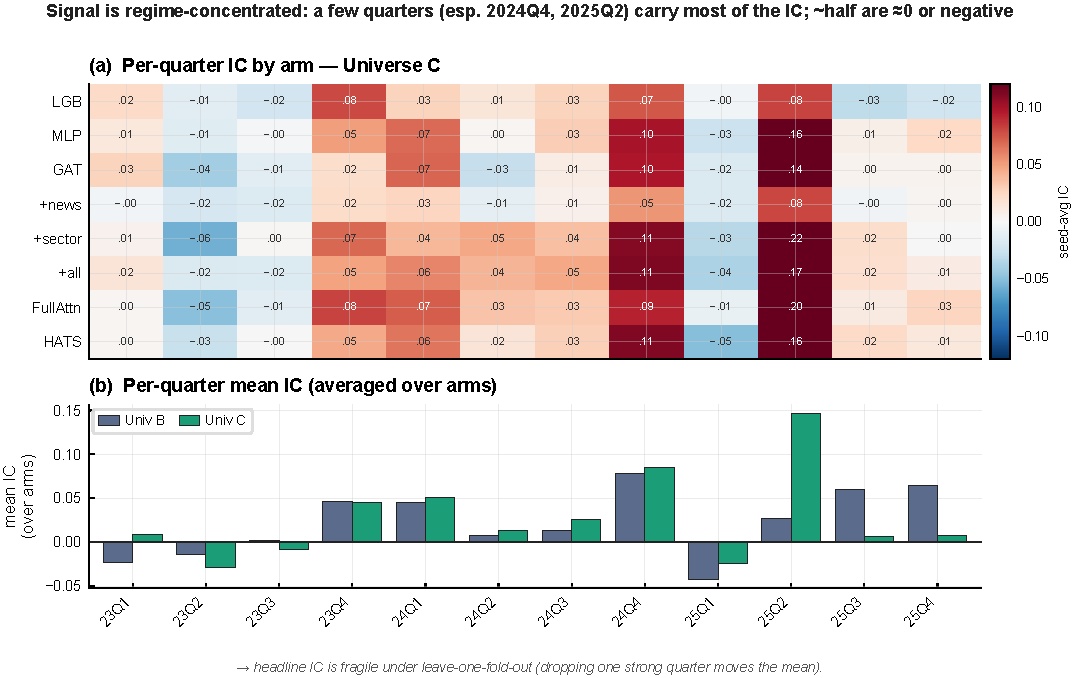
\includegraphics[width=\textwidth]{regime_perfold_ic}
  \caption{Per-fold IC by arm (descriptive companion to the pooled contrasts). (a)~Heatmap of seed-averaged IC for the tuned ladder arms across the 12 walk-forward quarters in Universe~C; (b)~per-quarter mean IC averaged over arms for Universes B and C. Degenerate C/L5s cells are excluded, matching the Family-1 handling (\S\ref{app:diag:stability}). The per-fold view explains why pooled IC levels are fragile under leave-one-fold-out, whereas the BH-rejected pairwise contrasts do not change sign in any leave-one-quarter-out replicate.}
  \label{app:diag:fig:regime}
\end{figure}

\subsection{Exploratory failure modes}\label{app:diag:exploratory}

% source: paper/main.tex, "Exploratory failure modes" subsection (reproduced verbatim)
The analyses in this subsection are outside the confirmatory families. In an earlier loss-function horse race, where MSE was later fixed for the confirmatory ladder, ListMLE showed a regime-shift inversion: per-cell mean IC was $-0.0458$, compared with $+0.0113$ for MSE. A plausible explanation is softmax likelihood overweighting the in-sample rank order, which can invert under regime shift. Figure~\ref{app:diag:fig:listmle} visualizes this inversion.

% source: paper/main.tex, "Exploratory failure modes" subsection (reproduced verbatim)
A separate issue is Universe-C's feature-basis leakage: only 5 of its 15 Plan-AAA Alpha158 groups survive strict $T-1$ re-ranking (Figure~\ref{app:diag:fig:planaaa}), so its positive results (MLP${}>{}$LightGBM, positive edge effects) are suggestive pending leak-free selection, while null and negative within-universe contrasts are less exposed (detailed in Limitation~L1).

\begin{figure}[t]
  \centering
  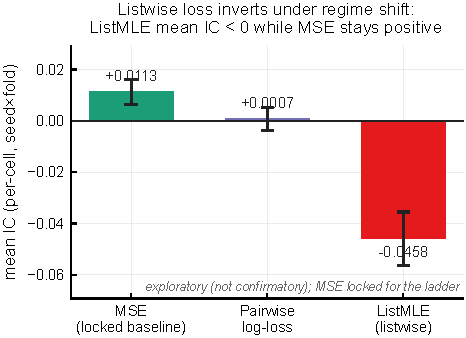
\includegraphics[width=.55\textwidth]{loss_listmle_inversion}
  % source: paper/main.tex, "Exploratory failure modes" subsection (−0.0458, +0.0113)
  \caption{ListMLE inversion in the loss-function horse race (exploratory, outside the confirmatory families). Mean per-cell IC by training loss, with $\pm 1$ standard error across cells. ListMLE's per-cell mean IC is $-0.0458$, against $+0.0113$ for MSE, the loss later fixed for the confirmatory ladder. A plausible explanation is softmax likelihood overweighting the in-sample rank order, which can invert under regime shift.}
  \label{app:diag:fig:listmle}
\end{figure}

\begin{figure}[t]
  \centering
  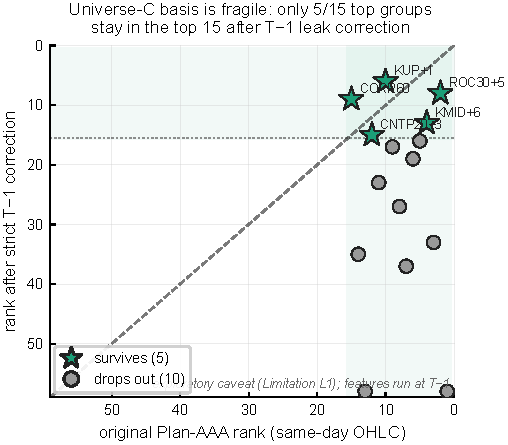
\includegraphics[width=.55\textwidth]{plan_aaa_t1_stability}
  % source: paper/main.tex, Limitations (L1) + "Exploratory failure modes" subsection (5 of 15)
  \caption{Plan-AAA feature-group ranking under strict $T-1$ re-ranking (exploratory, outside the confirmatory families). Original rank versus $T-1$-corrected proxy rank for the top-15 Alpha158 groups that define Universe~C's feature basis; only 5 of the 15 groups remain in the top 15. Runtime features are measured at $T-1$; it is the basis \emph{selection} that is leaked, so Universe-C positive results are suggestive pending leak-free re-selection (Limitation~L1).}
  \label{app:diag:fig:planaaa}
\end{figure}


\end{document}
